\documentclass[a4paper,12pt,oneside]{report}
\usepackage[english]{../../../../latex-setup/learningnotes}
\usepackage{needspace}
\usepackage{pgfplots}
\pgfplotsset{compat=1.18}
\hypersetup{linktoc=all}
\newcommand{\exerciseheading}[1]{%
  \par\Needspace{5\baselineskip}\noindent\textbf{#1}\par\nobreak}
\newcommand{\solutionheading}[1]{%
  \par\Needspace{5\baselineskip}\noindent
  \begingroup\setlength{\fboxsep}{1pt}%
  \colorbox{yellow}{\strut\textbf{#1}}\endgroup\par\nobreak}

\notestitle{FDS}
\notessubtitle{Fundamentals of Data Science}
\notesauthor{Matteo}
\notesdate{\today}

\begin{document}

\makenotestitle
\notescontents

\chapter{Introduction}

\begin{tcolorbox}[colback=yellow!20,colframe=yellow!60!black,
  boxrule=0.4pt,arc=1mm,left=5pt,right=5pt,top=3pt,bottom=3pt,
  before skip=0pt,after skip=0pt]
\small\textbf{Start of lecture 00 (Spinelli)}
\end{tcolorbox}

\section{What is Data Science?}

\begin{frameddefn}{Data Science}\label{def:data-science}
Data Science is an interdisciplinary field that extracts knowledge from
data to support decisions. It combines statistics, mathematics, computer
science, and domain expertise to collect, clean, manage, and analyse data.
\end{frameddefn}

\Needspace{24\baselineskip}
\section{The Data Science lifecycle}

A project moves through business understanding, data engineering,
model engineering, deployment, and monitoring. This cycle can repeat
when new data or retraining is needed.

\begin{center}
  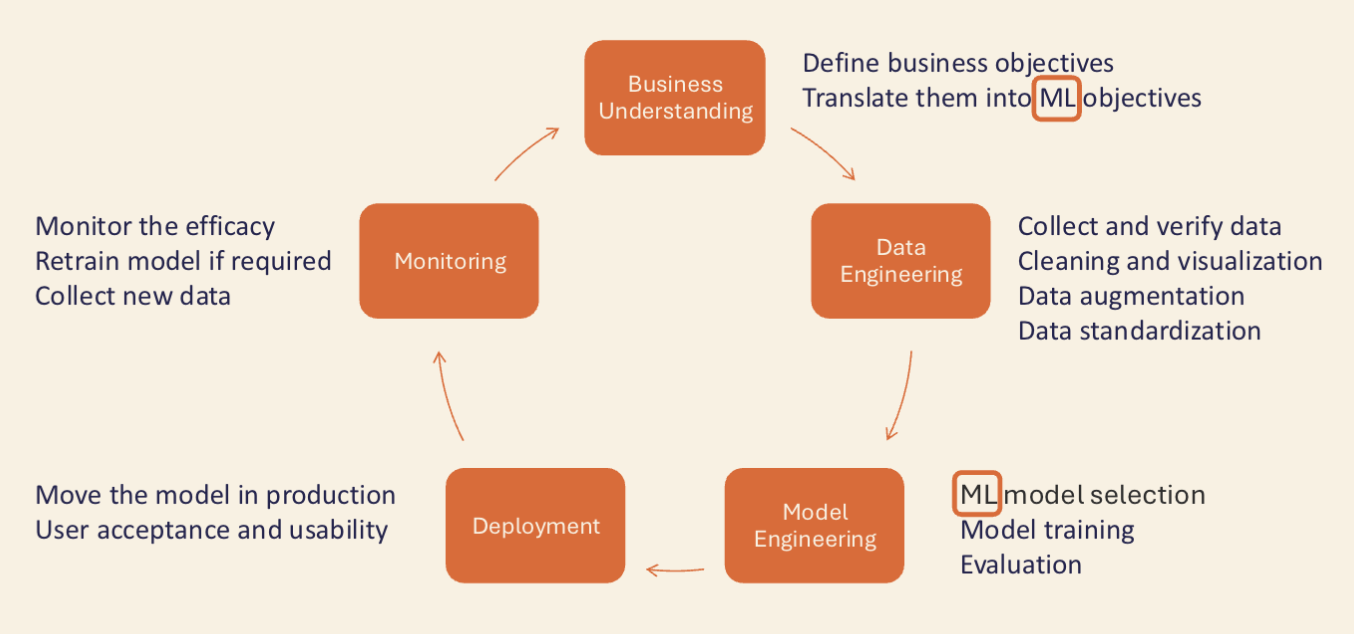
\includegraphics[width=0.95\linewidth]{assets/data-science-lifecycle.png}
  \par\smallskip
  {\small\textit{The Data Science lifecycle. Source: Spinelli, Lecture 00.}}
\end{center}

\clearpage
\section{Artificial Intelligence and Machine Learning}

\emph{Artificial Intelligence} (AI) studies how to build systems that
perform tasks requiring abilities such as reasoning, learning, and
problem solving.

\begin{frameddefn}{Machine Learning}\label{def:machine-learning}
Machine Learning (ML) studies algorithms whose performance $P$ on a task
$T$ improves through experience $E$. A learning problem therefore
specifies the task, the performance measure, and the available experience.
\end{frameddefn}

The main learning settings are:
\begin{itemize}
  \item \textbf{Supervised learning:} learn from inputs paired with known
        desired outputs to predict the output for new inputs.
  \item \textbf{Unsupervised learning:} discover structure in data without
        given target outputs.
  \item \textbf{Reinforcement learning:} learn how to act through
        interaction with an environment and feedback in the form of rewards.
\end{itemize}

\begin{center}
  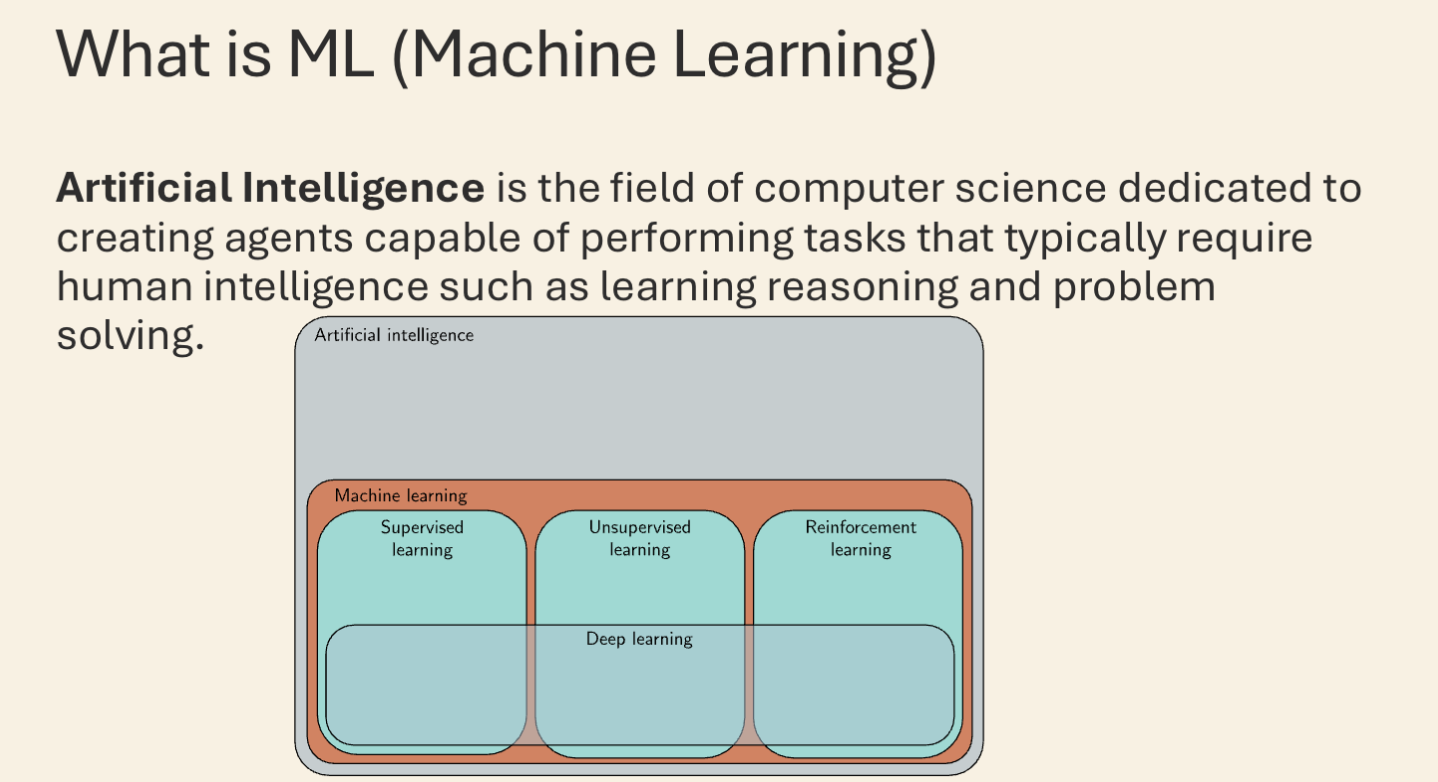
\includegraphics[width=\linewidth]{assets/artificial-intelligence-and-machine-learning.png}
  \par\smallskip
  {\small\textit{AI, ML, and learning settings. Source: Spinelli, Lecture 00.}}
\end{center}

\emph{Deep learning} uses neural networks with multiple layers and can
be applied in each of these settings.

\clearpage
\section{Supervised models and prediction tasks}

\begin{frameddefn}{Supervised learning model}\label{def:supervised-model}
A supervised learning model is a function
$f:\mathcal{X}\to\mathcal{Y}$ that maps an input $x$ to a predicted
output $\hat{y}=f(x)$. Here, $\mathcal{X}$ is the input space and
$\mathcal{Y}$ is the output space. Training means choosing or adjusting
$f$ using examples of inputs paired with their known outputs.
\end{frameddefn}

\begin{frameddefn}{Regression}\label{def:regression}
Regression is a supervised learning task whose target is a real-valued
number or vector. For example, predicting a person's height from their
age is a regression task.
\end{frameddefn}

\begin{frameddefn}{Classification}\label{def:classification}
Classification is a supervised learning task whose target is a category
from a finite set of classes. For example, predicting whether a flower
is setosa, versicolor, or virginica is a classification task.
\end{frameddefn}

\chapter{Data Representation}

\begin{tcolorbox}[colback=yellow!20,colframe=yellow!60!black,
  boxrule=0.4pt,arc=1mm,left=5pt,right=5pt,top=3pt,bottom=3pt,
  before skip=0pt,after skip=0pt]
\small\textbf{Start of lecture 01 (Spinelli) --- 2 October 2026}
\end{tcolorbox}

\section{The Iris dataset}

The Iris dataset contains 150 flowers, divided into three species:
50 setosa, 50 versicolor, and 50 virginica. The goal is to predict a
flower's species from its measurements.

\begin{framedexample}{Iris as a supervised classification task}
Each \textbf{observation} is one flower, described by four
\textbf{features}, all measured in centimetres:
\begin{itemize}
  \item sepal length and sepal width;
  \item petal length and petal width.
\end{itemize}
The \textbf{target} is the flower's species. This is supervised learning
because the species is known for the training examples, and
classification because the target is a category.
\end{framedexample}

\clearpage
\section{Features and targets}

In a tabular dataset, each row describes one observation. The feature
columns contain its input measurements, while the target column contains
the output we want to predict.

For the first flower shown in the lecture's table,
\[
  x=(4.3,\;3.0,\;1.1,\;0.1),
  \qquad y=\text{setosa}.
\]
The entries of $x$ are, in order, sepal length, sepal width, petal length,
and petal width, all in centimetres.

During training, both $x$ and $y$ are known. For a new input $x$, the model
produces a prediction $\hat{y}=f(x)$. The observed target $y$ and the
predicted target $\hat{y}$ may differ.

\section{Data types}

Features and targets can have different types:
\begin{center}
\begin{tabularx}{\linewidth}{@{}llX@{}}
\toprule
\textbf{Type} & \textbf{Values} & \textbf{Example} \\
\midrule
Real-valued & $\mathbb{R}$ & Petal length \\
Integer-valued & $\mathbb{Z}$ & Number of purchases \\
Categorical & $\{C_1,\ldots,C_g\}$ & Flower species \\
Binary & $\{0,1\}$ & Spam or non-spam \\
\bottomrule
\end{tabularx}
\end{center}

Predicting a numerical quantity is a regression task; predicting a
category is a classification task. In Iris, the four features are
numerical measurements and the target has three categories.

Assigning codes $0,1,2$ to the species does not turn them into numerical
quantities: the codes identify categories, so the task remains
classification.

% Spinelli, Lecture 01: data_vectors.
\clearpage
\section{Encoding categorical features}

How can we give a colour to a model that works with numbers? Many learning
algorithms require numerical features, so we need an \emph{encoding}: a
way to represent a category using numbers.

We could assign the codes red $=0$, green $=1$, and blue $=2$. But a model
that treats these codes as quantities could interpret blue as greater
than green, or as twice as far from red as green is. Colours have no
such order, and these numerical distances have no meaning here.

\emph{One-hot encoding} replaces the colour column with three yes/no
questions: ``Is it red?'', ``Is it green?'', and ``Is it blue?''.
We use $1$ for yes and $0$ for no.

\begin{framedexample}{Encoding a colour feature}
\begin{center}
\begin{tabular}{@{}lccc@{}}
\toprule
\textbf{Colour} & \textbf{Is it red?} & \textbf{Is it green?} & \textbf{Is it blue?} \\
\midrule
Red   & $1$ & $0$ & $0$ \\
Green & $0$ & $1$ & $0$ \\
Blue  & $0$ & $0$ & $1$ \\
\bottomrule
\end{tabular}
\end{center}
For example, a green product is represented by $(0,1,0)^\top$.
Exactly one entry is $1$ and all the others are $0$: this is why the
encoding is called \emph{one-hot}.
\end{framedexample}

A model predicting a product's price can then learn a separate effect
for each colour, without assuming that blue is ``twice'' green.
The cost is more columns: one feature with $k$ categories becomes $k$
numerical columns. We can now write this idea formally.

\begin{frameddefn}{One-hot encoding}\label{def:one-hot}
For a feature with $k$ mutually exclusive categories, one-hot encoding
represents category $C_i$ by a vector $e_i\in\{0,1\}^{k}$ whose $i$-th
entry is $1$ and whose other entries are $0$:
\[
  (e_i)_j=\begin{cases}
    1,&j=i,\\
    0,&j\neq i.
  \end{cases}
\]
Each observation belongs to exactly one category, so its encoded vector
has exactly one nonzero entry.
\end{frameddefn}

When categories have a natural order, an \emph{ordinal encoding} can
preserve it. For example, low, medium, and high can be coded as $0,1,2$.
This expresses their order; it does not establish that the gaps between
successive categories are equal.

\section{Labels}

\begin{frameddefn}{Labels and labeled data}\label{def:labels}
A \emph{label} is an observed target value. In \emph{labeled data}, the
input and its target are both available.\newline
In \emph{unlabeled data}, the
input is available but its target is unknown or unrecorded.
\end{frameddefn}

In Iris, a flower with measurements and a known species is labeled;
the same measurements without the species are unlabeled. A label can
also be numerical, as in a regression task.

\clearpage
\section{Dataset notation}

Let $n$ be the number of observations and $p$ the number of numerical
features after any encoding. Write $\mathcal{X}\subseteq\mathbb{R}^{p}$
for the input space and $\mathcal{Y}$ for the target space.

\begin{frameddefn}{Supervised dataset}\label{def:dataset}
A labeled dataset is an indexed collection of input--target pairs,
\[
  D=\bigl((x^{(1)},y^{(1)}),\ldots,(x^{(n)},y^{(n)})\bigr)
    \in(\mathcal{X}\times\mathcal{Y})^{n}.
\]
The $i$-th observation has an input column vector
\[
  x^{(i)}=(x_1^{(i)},\ldots,x_p^{(i)})^\top\in\mathbb{R}^{p}
\]
and a target $y^{(i)}\in\mathcal{Y}$.
\end{frameddefn}

The superscript $(i)$ indexes an observation; the subscript $j$ indexes
a feature. Across all observations, the $j$-th feature column is
\[
  \mathbf{x}_j=(x_j^{(1)},\ldots,x_j^{(n)})^\top\in\mathbb{R}^{n}.
\]
Thus an input vector contains $p$ features of one observation, while a
feature column contains $n$ values of one feature.

\begin{framedexample}{A small supervised dataset}
Suppose we predict house prices from area and room count. Here is a toy dataset:
\begin{center}
\begin{tabular}{@{}cccc@{}}
\toprule
\textbf{House $i$} & \textbf{Area ($\mathrm{m}^2$)} & \textbf{Rooms} & \textbf{Price (EUR)} \\
\midrule
$1$ & $50$  & $2$ & $150\,000$ \\
$2$ & $80$  & $3$ & $240\,000$ \\
$3$ & $100$ & $4$ & $300\,000$ \\
\bottomrule
\end{tabular}
\end{center}
Here $n=3$ houses and $p=2$ input features. The price is the target,
so it is not counted in $p$. For the first house,
\[
  x^{(1)}=(50,2)^\top,
  \qquad y^{(1)}=150\,000.
\]
$D$ collects the three input--target pairs. Here $x_2^{(1)}=2$ is the
first house's room count. The rooms column is
\[
  \mathbf{x}_2=(2,3,4)^\top.
\]
The vector $x^{(1)}$ describes one house using both features; the vector
$\mathbf{x}_2$ contains one feature for all three houses.
\end{framedexample}

\section{Data generation and the i.i.d. assumption}

We model the observations as realizations of random pairs $(X,Y)$
with an unknown joint probability distribution $P_{XY}$ on
$\mathcal{X}\times\mathcal{Y}$. Capital letters denote random variables;
lowercase letters denote their observed values. Supervised learning
uses these observations to learn a predictive relationship between
input and target.

\begin{frameddefn}{I.i.d. observations}
\label{def:iid}
The observations are \emph{i.i.d.} when their random pairs
$(X^{(1)},Y^{(1)}),\ldots,(X^{(n)},Y^{(n)})$ are mutually independent
and all have the same distribution $P_{XY}$.
\end{frameddefn}

Independence is between observations; it does not require $X$ and $Y$
within one observation to be independent. The i.i.d. assumption can fail,
for example when successive observations form a time series.

\begin{notebox}[Notation from the next section on]
From the next section on we follow the notation of the slides, which
comes from \emph{Machine Learning Refined}. Each input has $N$
coordinates and the dataset contains $P$ points: compared with the
notation above, $N=p$ and $P=n$.
\begin{itemize}
  \item $x_p\in\mathbb{R}^{N}$ is the $p$-th point, for $p=1,\ldots,P$.
  \item For a single vector without a point index, such as $u$ or $x$,
        the subscripts $1,\ldots,N$ number its coordinates, as in the
        axis labels $x_1,x_2$ of the figures.
  \item When both indices are needed, $x_{n,p}$ is coordinate $n$ of the
        point $x_p$.
\end{itemize}
\end{notebox}

\clearpage
\section{Data points as vectors}

We now focus on the inputs $x_p\in\mathbb{R}^{N}$. This space
supports vector addition and multiplication by real numbers, called
\emph{scalars}. These operations act coordinate by coordinate:
\[
  u+v=(u_1+v_1,\ldots,u_N+v_N)^\top,
  \qquad
  a u=(a u_1,\ldots,a u_N)^\top.
\]
An input can be drawn as a point with those coordinates or as a
\emph{position vector}: an arrow from the origin to that point.

\subsection{Mean-centering}

\begin{frameddefn}{Mean-centered data}\label{def:mean-centering}
The sample mean input vector and the centered observations are
\[
  \bar{x}=\frac{1}{P}\sum_{p=1}^{P}x_p,
  \qquad
  \widetilde{x}_p=x_p-\bar{x}.
\]
The mean of the centered inputs is zero:
$\frac{1}{P}\sum_{p=1}^{P}\widetilde{x}_p=0$.
\end{frameddefn}

Centering subtracts each feature's sample mean from that feature. It is
reversible if we retain $\bar{x}$, since
$x_p=\widetilde{x}_p+\bar{x}$.

\begin{framedexample}{Centering three points}
For the inputs $(1,1)^\top$, $(3,1)^\top$, and $(2,4)^\top$,
\[
  \bar{x}=\left(\frac{1+3+2}{3},\frac{1+1+4}{3}\right)^\top
         =(2,2)^\top.
\]
The centered inputs are $(-1,-1)^\top$, $(1,-1)^\top$, and
$(0,2)^\top$. Their sum is $(0,0)^\top$.
\end{framedexample}

\begin{center}
\begin{tikzpicture}[x=0.85cm,y=0.85cm,font=\small]
  \foreach \shift/\heading in {0/Points,6/Position vectors}{
    \begin{scope}[xshift=\shift cm]
      \draw[step=1,black!15,very thin] (-2,-2) grid (2,3);
      \draw[-{Stealth},black!60] (-2,0)--(2.3,0) node[right] {$x_1$};
      \draw[-{Stealth},black!60] (0,-2)--(0,3.3) node[above] {$x_2$};
      \node[above left] at (0,0) {$0$};
      \node[above] at (0,3.7) {\heading};
      \foreach \px/\py in {-1/-1,1/-1,0/2}{
        \ifnum\shift=0
          \fill[NotesBlue] (\px,\py) circle (2pt);
        \else
          \draw[-{Stealth},NotesBlue,thick] (0,0)--(\px,\py);
        \fi
      }
    \end{scope}
  }
\end{tikzpicture}
\par\smallskip
{\small\textit{The same centered observations, drawn as points and as arrows.}}
\end{center}

\clearpage
\section{Spanning sets}

\begin{frameddefn}{Span and spanning set}\label{def:span}
The \emph{span} of vectors $c_1,\ldots,c_K$ is the set of all their
linear combinations:
\[
  \operatorname{span}\{c_1,\ldots,c_K\}
  =\left\{\sum_{n=1}^{K}a_nc_n:a_1,\ldots,a_K\in\mathbb{R}\right\}.
\]
These vectors form a \emph{spanning set} of a vector space $V$ when
their span equals $V$: every vector in $V$ can be expressed using them.
\end{frameddefn}

\begin{framedexample}{Spanning the plane}
The vectors
\[
  e_1=\begin{pmatrix}1\\0\end{pmatrix},\qquad
  e_2=\begin{pmatrix}0\\1\end{pmatrix}
\]
span $\mathbb{R}^{2}$, because every $(a,b)^\top$ can be written as
$a e_1+b e_2$. For example,
\[
  \begin{pmatrix}2\\3\end{pmatrix}=2e_1+3e_2.
\]
\begin{center}
\begin{tikzpicture}[x=1cm,y=1cm,font=\small]
  \draw[step=1,black!15,very thin] (-0.5,-0.5) grid (3,4);
  \draw[-{Stealth},black!60] (-0.5,0)--(3.4,0);
  \draw[-{Stealth},black!60] (0,-0.5)--(0,4.2);
  \draw[-{Stealth},NotesBlue,thick] (0,0)--(2,0)
    node[midway,below] {$2e_1$};
  \draw[-{Stealth},NotesBlue,thick] (2,0)--(2,3)
    node[midway,right] {$3e_2$};
  \draw[-{Stealth},black,thick] (0,0)--(2,3)
    node[midway,above left] {$x$};
  \node[above right] at (2,3) {$(2,3)$};
  \node[below left] at (0,0) {$0$};
\end{tikzpicture}
\end{center}
Using only $e_1$ produces vectors $(a,0)^\top$, so it spans the
horizontal axis rather than the whole plane.
\end{framedexample}

\clearpage
\section{Basis}

\begin{frameddefn}{Linear independence}\label{def:linear-independence}
Vectors $c_1,\ldots,c_K\in\mathbb{R}^{N}$ are \emph{linearly independent}
if the only scalars $a_1,\ldots,a_K\in\mathbb{R}$ satisfying
\[
  a_1c_1+\cdots+a_Kc_K=0
\]
are $a_1=\cdots=a_K=0$.
\end{frameddefn}

\begin{frameddefn}{Basis}\label{def:basis}
A \emph{basis} of a vector space is a linearly independent spanning
set. Equivalently, it is a minimal spanning set: removing any of its
vectors destroys the spanning property.
\end{frameddefn}

\begin{framedexample}{A spanning set with a redundant vector}
The pair $\{e_1,e_2\}$ is a basis of $\mathbb{R}^{2}$. Adding
$c_3=e_1+e_2$ still gives a spanning set, but it is not a basis, since
\[
  e_1+e_2-c_3=0
\]
is a linear combination with nonzero coefficients. The third vector
is redundant because the first two already generate it.
\end{framedexample}

\subsection{Representing observations in a basis}

A basis of $\mathbb{R}^{N}$ contains exactly $N$ vectors, each in
$\mathbb{R}^{N}$. For a basis $c_1,\ldots,c_N$, every input observation
has a unique representation
\[
  x_p=\sum_{n=1}^{N}w_{n,p}c_n,
  \qquad p=1,\ldots,P.
\]
The coefficients $w_{n,p}$ are the \emph{weights}, or coordinates,
of that observation in the chosen basis. The vector
$w_p=(w_{1,p},\ldots,w_{N,p})^\top$ records its representation;
combining the basis vectors with these weights reconstructs $x_p$.

\Needspace{28\baselineskip}
\begin{framedexample}{Coordinates in a basis}
Use the same basis for both observations:
\[
  c_1=\begin{pmatrix}1\\0\end{pmatrix},\qquad
  c_2=\begin{pmatrix}0\\1\end{pmatrix}.
\]
The two points have different weights:
\[
\begin{aligned}
  x_1&=\begin{pmatrix}2\\3\end{pmatrix}=2c_1+3c_2,\\[4pt]
  x_2&=\begin{pmatrix}4\\1\end{pmatrix}=4c_1+c_2.
\end{aligned}
\]
\begin{center}
\begin{tabular}{@{}lll@{}}
\toprule
\textbf{Observation} & \textbf{Weight of $c_1$} & \textbf{Weight of $c_2$} \\
\midrule
First ($p=1$) & $w_{1,1}=2$ & $w_{2,1}=3$ \\
Second ($p=2$) & $w_{1,2}=4$ & $w_{2,2}=1$ \\
\bottomrule
\end{tabular}
\end{center}
For example, $w_{2,1}=3$ means that the first observation uses three
times the second basis vector. In $w_{n,p}$, the first index $n$ identifies the
basis vector; the second index $p$ identifies the observation.
\end{framedexample}

\clearpage
\section{Standard basis}

\begin{frameddefn}{Standard basis}\label{def:standard-basis}
The \emph{standard basis} of $\mathbb{R}^{N}$ consists of the vectors
$c_1,\ldots,c_N$, where $c_n$ has a $1$ in position $n$ and zeros
everywhere else. In $\mathbb{R}^{2}$,
\[
  c_1=\begin{pmatrix}1\\0\end{pmatrix},\qquad
  c_2=\begin{pmatrix}0\\1\end{pmatrix}.
\]
\end{frameddefn}

Each vector points along one coordinate axis. Consequently, the weights
in this basis are the entries of the observation itself:
\[
  x_p=x_{1,p}c_1+\cdots+x_{N,p}c_N
  \qquad\Longrightarrow\qquad w_p=x_p.
\]

\begin{framedexample}{Reading the weights from the coordinates}
For $x=(2,3)^\top$, move two units along the first axis and three along
the second:
\[
  x=2c_1+3c_2,\qquad w=\begin{pmatrix}2\\3\end{pmatrix}=x.
\]
\begin{center}
\begin{tikzpicture}[font=\small]
  \begin{scope}[x=1.55cm,y=1.55cm]
    \node[font=\small\bfseries] at (0.6,2.15) {Unit basis vectors};
    \draw[-{Stealth},black!50] (-0.3,0)--(1.6,0);
    \draw[-{Stealth},black!50] (0,-0.3)--(0,1.7);
    \draw[-{Stealth},NotesBlue,very thick] (0,0)--(1,0)
      node[below] {$c_1=(1,0)^\top$};
    \draw[-{Stealth},red!65!black,very thick] (0,0)--(0,1)
      node[above right] {$c_2=(0,1)^\top$};
    \draw[black!50] (0.16,0)--(0.16,0.16)--(0,0.16);
    \node[below left] at (0,0) {$0$};
  \end{scope}
  \begin{scope}[shift={(5.1cm,0)},x=0.85cm,y=0.85cm]
    \node[font=\small\bfseries] at (1.25,3.92) {Representing $x=(2,3)^\top$};
    \draw[step=1,black!12,very thin] (0,0) grid (3,3);
    \draw[-{Stealth},black!50] (-0.35,0)--(3.2,0);
    \draw[-{Stealth},black!50] (0,-0.35)--(0,3.55);
    \draw[-{Stealth},NotesBlue,very thick] (0,0)--(2,0)
      node[midway,below] {$2c_1$};
    \draw[-{Stealth},red!65!black,very thick] (2,0)--(2,3)
      node[midway,right] {$3c_2$};
    \draw[-{Stealth},black,thick] (0,0)--(2,3)
      node[midway,above left] {$x$};
    \node[above right] at (2,3) {$(2,3)$};
    \node[below left] at (0,0) {$0$};
  \end{scope}
\end{tikzpicture}
\end{center}
The blue arrow contributes the first coordinate; the red arrow
contributes the second. Their sum is the black arrow.
\end{framedexample}

\clearpage
\subsection{Orthogonality, unit length, and the basis matrix}

The standard basis has two properties:
\begin{itemize}
  \item \textbf{Different vectors are perpendicular:}
        $c_n^\top c_m=0$ for $n\ne m$.
  \item \textbf{Each vector has unit length:}
        $\lVert c_n\rVert_2^2=c_n^\top c_n=1$.
\end{itemize}
In $\mathbb{R}^{2}$, these follow directly from
\[
  c_1^\top c_2=1\cdot0+0\cdot1=0,\qquad
  \lVert c_1\rVert_2^2=1^2+0^2=1,
\]
and similarly $\lVert c_2\rVert_2^2=1$.

\begin{frameddefn}{Orthonormal basis}\label{def:orthonormal-basis}
A basis is \emph{orthonormal} if its vectors are mutually perpendicular
and each has length $1$.
\end{frameddefn}

How can we check whether a basis is orthonormal? We need to check the
length of every vector and whether each pair of different vectors is
perpendicular. With many vectors, drawing arrows is impractical. We
can collect all these checks in one matrix.

First, place the basis vectors in the columns of $C$:
\[
  C=[\,c_1\ \cdots\ c_N\,]
  \in\mathbb{R}^{N\times N}.
\]
Now compute $C^\top C$. Each entry is a dot product between two columns
of $C$: the entry in row $n$, column $m$ is $c_n^\top c_m$.
We read the result as a table of checks:
\begin{center}
\begin{tabularx}{\linewidth}{@{}lXc@{}}
\toprule
\textbf{Position} & \textbf{What it tells us} & \textbf{Required value} \\
\midrule
On the diagonal & A vector's length squared & $1$ \\
Off the diagonal & The dot product of two different vectors & $0$ \\
\bottomrule
\end{tabularx}
\end{center}

If the diagonal contains only $1$s and every other entry is $0$, both
checks pass: the basis is orthonormal. That result is the identity
matrix $I_N$ (written $I_{N\times N}$ in the slides), so the complete test is
\[
  \boxed{C^\top C=I_N.}
\]
This formula is a compact way to check the lengths and perpendicularity
of all the basis vectors at once. The standard basis passes the test.

\Needspace{22\baselineskip}
\begin{framedexample}{Using the orthonormality test}
Consider the basis
\[
  c_1=\begin{pmatrix}1\\0\end{pmatrix},\qquad
  c_2=\begin{pmatrix}0.6\\0.8\end{pmatrix},\qquad
  C=\begin{pmatrix}1&0.6\\0&0.8\end{pmatrix}.
\]
Both vectors have length $1$, since $1^2+0^2=1$ and
$0.6^2+0.8^2=1$. Do they also pass the perpendicularity check?
\[
  C^\top C
  =\begin{pmatrix}
     1&0\\0.6&0.8
   \end{pmatrix}
   \begin{pmatrix}1&0.6\\0&0.8\end{pmatrix}
  =\begin{pmatrix}1&0.6\\0.6&1\end{pmatrix}.
\]
The diagonal $1$s confirm the unit lengths. The off-diagonal entries
are $0.6$, so the vectors are not perpendicular. Therefore
$C^\top C\ne I_2$: this basis is not orthonormal, even though both
vectors have length $1$.
\end{framedexample}

In the standard basis, the weights equal the entries of the observation:
$w=x$. For a different orthonormal basis, the same observation can have
different weights. The test $C^\top C=I_N$ checks the geometry of the
basis; the chosen basis determines the weights.

\clearpage
\section{Coordinates in an orthonormal basis}

We now know how to check a basis. How do we find the weights needed to
represent a point in that basis? For an orthonormal basis, a dot product
with each basis vector gives the answer.

We know the observation $x$ and choose the basis vectors
$c_1,\ldots,c_N$. We want to find their weights $w_1,\ldots,w_N$ so that
their weighted sum gives $x$. Put the basis vectors in the columns of
$C$ and the weights in $w$. Matrix multiplication performs that sum:
\[
  Cw=w_1c_1+\cdots+w_Nc_N=x.
\]
Thus $x=Cw$ is the compact form of a linear combination. Multiplying
both sides by $C^\top$ gives
\[
  C^\top x=C^\top Cw=I_Nw=w.
\]
Therefore the coordinates are
\[
  \boxed{w=C^\top x,\qquad w_n=c_n^\top x.}
\]
The weight $w_n$ tells us how far to move along the unit vector $c_n$.
A positive weight follows its direction; a negative weight goes in the
opposite direction. Perpendicular basis vectors do not contribute to
this dot product, so it picks out just the weight we want.

For every observation $x_p$, the same calculation gives
$w_p=C^\top x_p$. With a complete orthonormal basis, combining
these weights with the basis vectors gives the original observation:
\[
  Cw_p=CC^\top x_p=x_p.
\]
Here $C$ is square and its columns form a basis of all of
$\mathbb{R}^N$, so $CC^\top=I_N$ as well as $C^\top C=I_N$.

\clearpage
\begin{framedexample}{Finding the weights of the point $(2,3)$}
Our observation is $x=(2,3)^\top$: two units to the right and three
units up. We want to describe this same point using two different
unit directions:
\[
  c_1=\begin{pmatrix}0\\1\end{pmatrix}
    \quad\text{(up)},\qquad
  c_2=\begin{pmatrix}-1\\0\end{pmatrix}
    \quad\text{(left)}.
\]
These vectors are perpendicular and have length $1$, so they form an
orthonormal basis. We seek weights $w_1,w_2$ for which
$x=w_1c_1+w_2c_2$.

\begin{center}
\begin{tikzpicture}[font=\small,x=1cm,y=1cm]
  \draw[step=1,black!12,very thin] (-1,0) grid (3,3);
  \draw[-{Stealth},black!50] (-1.2,0)--(3.3,0) node[right] {$x_1$};
  \draw[-{Stealth},black!50] (0,-0.3)--(0,3.65) node[above] {$x_2$};
  \draw[-{Stealth},NotesBlue,very thick] (0,0)--(0,3)
    node[midway,left] {$3c_1$: 3 units up};
  \draw[-{Stealth},red!65!black,very thick] (0,3)--(2,3)
    node[midway,above,align=center,xshift=0.3cm] {$-2c_2$\\2 units right};
  \draw[-{Stealth},black,thick] (0,0)--(2,3)
    node[midway,below right] {$x$};
  \fill (2,3) circle (2pt) node[right] {$x=(2,3)^\top$};
  \node[below left] at (0,0) {$0$};
\end{tikzpicture}
\end{center}

Read the two moves in the drawing:
\begin{itemize}
  \item Along $c_1$, we need to go up three units, so $w_1=3$.
  \item $c_2$ points left, but we need to go right two units. We move
        against its direction, so $w_2=-2$.
\end{itemize}
The dot-product rule gives exactly these weights:
\[
\begin{aligned}
  w_1&=c_1^\top x=0\cdot2+1\cdot3=3,\\
  w_2&=c_2^\top x=(-1)\cdot2+0\cdot3=-2.
\end{aligned}
\]
Thus $w=(3,-2)^\top$. To check these weights, add their contributions:
\[
  Cw=3c_1-2c_2
    =\begin{pmatrix}0\\3\end{pmatrix}
     +\begin{pmatrix}2\\0\end{pmatrix}
    =\begin{pmatrix}2\\3\end{pmatrix}=x.
\]
The sum gives our original observation. Its weights are $(2,3)$ in
the standard basis and $(3,-2)$ in the chosen basis. Both sets of
weights describe the same point using their respective basis vectors.
\end{framedexample}

\clearpage
\section{Nonstandard bases}

The standard basis is convenient, but we can choose other directions.
They must be linearly independent and span the space; they do not have
to be perpendicular or have unit length.

Consider the basis from the slides:
\[
  c_1=\begin{pmatrix}2\\1\end{pmatrix},\qquad
  c_2=\begin{pmatrix}1\\2\end{pmatrix},\qquad
  C=\begin{pmatrix}2&1\\1&2\end{pmatrix}.
\]
The vectors are independent, but $c_1^\top c_2=4$ and each has length
$\sqrt{5}$. This basis is not orthonormal.

To find the weights, we must still solve $Cw=x$.

\Needspace{28\baselineskip}
\begin{framedexample}{Representing $(5,5)$ in a different basis}
For $x=(5,5)^\top$, the equation $w_1c_1+w_2c_2=x$ becomes
\[
  \begin{cases}
    2w_1+w_2=5,\\
    w_1+2w_2=5.
  \end{cases}
\]
Solving the system gives $w_1=w_2$, so
\[
  w_1=w_2=\frac{5}{3},\qquad
  x=\frac{5}{3}c_1+\frac{5}{3}c_2.
\]
\begin{center}
\begin{tikzpicture}[font=\small]
  \begin{scope}[x=0.62cm,y=0.62cm]
    \node[font=\small\bfseries] at (2.5,7.1) {Original coordinates};
    \draw[step=1,black!12,very thin] (0,0) grid (5,5);
    \draw[-{Stealth},black!50] (-0.3,0)--(5.9,0) node[right] {$x_1$};
    \draw[-{Stealth},black!50] (0,-0.3)--(0,5.8) node[above] {$x_2$};
    \draw[-{Stealth},NotesBlue,very thick] (0,0)--(3.333,1.667)
      node[midway,below right] {$(5/3)c_1$};
    \draw[-{Stealth},red!65!black,very thick] (3.333,1.667)--(5,5)
      node[midway,right] {$(5/3)c_2$};
    \draw[-{Stealth},black,thick] (0,0)--(5,5)
      node[midway,above left] {$x$};
    \fill (5,5) circle (2pt) node[above right] {$(5,5)$};
    \node[below left] at (0,0) {$0$};
  \end{scope}
  \begin{scope}[shift={(7.1cm,0)},x=1.15cm,y=1.15cm]
    \node[font=\small\bfseries] at (0.9,3.83) {New coordinates};
    \draw[-{Stealth},black!50] (-0.2,0)--(2.65,0) node[right] {$w_1$};
    \draw[-{Stealth},black!50] (0,-0.2)--(0,2.75) node[above] {$w_2$};
    \draw[dashed,black!45] (1.667,0)--(1.667,1.667)--(0,1.667);
    \draw[-{Stealth},NotesBlue,thick] (0,0)--(1.667,1.667);
    \fill[NotesBlue] (1.667,1.667) circle (2pt)
      node[above right] {$w$};
    \node[below] at (1.667,0) {$5/3$};
    \node[left] at (0,1.667) {$5/3$};
    \node[below left] at (0,0) {$0$};
  \end{scope}
\end{tikzpicture}
\end{center}
On the left, the two contributions add up to the original point.
On the right, we record their weights: $w=(5/3,5/3)^\top$.
\end{framedexample}

\Needspace{15\baselineskip}
\subsection{Encoding and decoding}

Here we use the same basis as in the previous example. Its two vectors
are the columns of the matrix $C$:
\[
  c_1=\begin{pmatrix}2\\1\end{pmatrix},\qquad
  c_2=\begin{pmatrix}1\\2\end{pmatrix},\qquad
  C=\begin{pmatrix}2&1\\1&2\end{pmatrix}.
\]
The vector $w=(w_1,w_2)^\top$ stores the two weights: how much of each
basis vector we need to add. Multiplying $C$ by $w$ performs this sum:
\[
  Cw=w_1c_1+w_2c_2.
\]
Thus $Cw$ is a point expressed in the original coordinates.

\emph{Encoding} means starting from a point $x$ and finding the weights
$w$ such that $Cw=x$. \emph{Decoding} means starting from the weights
$w$ and computing $Cw$ to obtain the point in its original coordinates.

For example, keep this same matrix $C$ and choose the weights
$w=(-2,1)^\top$. Decoding gives
\[
  Cw=-2c_1+c_2
  =-2\begin{pmatrix}2\\1\end{pmatrix}
   +\begin{pmatrix}1\\2\end{pmatrix}
  =\begin{pmatrix}-3\\0\end{pmatrix}.
\]
These weights describe the point $x=(-3,0)^\top$. The weight $-2$ means
taking twice $c_1$ in the opposite direction; the weight $1$ means adding
one copy of $c_2$.

Because these vectors form a basis, each point has exactly one pair of
weights. Encoding a point and then decoding its weights returns that
same point.

\Needspace{8\baselineskip}
\section{Finding the weights by least squares}

We know the point $x$ and the basis matrix $C$. We want to find the
weights $w$ with which to combine the columns of $C$. Each choice of
weights produces a point $Cw$. Our question is:
\emph{which weights make this point as close as possible to $x$?}

Start with the basis and point from the previous example:
\[
  C=\begin{pmatrix}2&1\\1&2\end{pmatrix},\qquad
  x=\begin{pmatrix}5\\5\end{pmatrix}.
\]
Suppose we try the weights $w=(1,1)^\top$. Adding one copy of each
basis vector gives
\[
  Cw=\begin{pmatrix}3\\3\end{pmatrix},\qquad
  Cw-x=\begin{pmatrix}-2\\-2\end{pmatrix}.
\]
We wanted $(5,5)$, but obtained $(3,3)$. The difference $Cw-x$ is the
\emph{reconstruction error}: how far off we are on each coordinate.
To measure it with a single number, square each coordinate error and
add the results. For these weights, the result is
\[
  (-2)^2+(-2)^2=8.
\]
Squaring makes each contribution nonnegative, so errors on different
coordinates cannot cancel each other.

For a point with $N$ coordinates, we call this sum $h(w)$:
\[
  h(w)=\lVert Cw-x\rVert_2^2
      =\sum_{n=1}^{N}\bigl((Cw)_n-x_n\bigr)^2.
\]
Here $(Cw)_n$ is the $n$th coordinate of the reconstructed point and
$x_n$ is the corresponding coordinate of the original point.
\emph{Least squares} means choosing the weights that make $h(w)$ as
small as possible.

With a complete basis, we can reconstruct $x$ exactly, so the minimum
error is zero. We will obtain the same weights as by solving $Cw=x$.
This formulation will also let us find the best approximation when
we keep fewer directions and exact reconstruction is impossible.

\Needspace{31\baselineskip}
\begin{framedexample}{Approximating a point with one direction}
Take the point $x=(2,3)^\top$: two units to the right and three units
up. Suppose we have only one direction: the horizontal vector
$c_1=(1,0)^\top$.
The matrix $C$ now has one column, and the weight $w$ is a single number:
\[
  C=\begin{pmatrix}1\\0\end{pmatrix},\qquad
  Cw=\begin{pmatrix}w\\0\end{pmatrix}.
\]
Every point we can reconstruct lies on the horizontal axis: its second
coordinate is always zero.

\begin{center}
\begin{tikzpicture}[x=0.9cm,y=0.9cm,font=\small]
  \draw[-{Stealth},black!40] (0,-0.3)--(0,3.7)
    node[above] {$x_2$};
  \draw[-{Stealth},NotesBlue,thick] (-0.4,0)--(3.7,0)
    node[right] {$x_1$};
  \draw[red!65!black,dashed,thick] (2,0)--(2,3)
    node[midway,right] {3 units};
  \fill (2,3) circle (2.5pt)
    node[above right] {$x=(2,3)^\top$};
  \fill[NotesBlue] (2,0) circle (2.5pt)
    node[below] {$(2,0)$};
  \node[below left] at (0,0) {$0$};
  \node[NotesBlue] at (1.7,-0.8) {Available points: $(w,0)$};
\end{tikzpicture}
\end{center}

The point $x$ is three units above the horizontal axis, so we cannot
reach it exactly. The closest available point is $(2,0)$, directly
below $x$, obtained by choosing $w=2$.

The squared reconstruction error is
\[
  h(w)=(w-2)^2+(0-3)^2=(w-2)^2+9.
\]
Choosing $w=2$ makes the first term zero. The minimum squared error
is therefore $9$.

We can also find the best weight by setting the derivative of $h$ to
zero:
\[
  h'(w)=2(w-2)=0
  \quad\Longrightarrow\quad w=2.
\]
\end{framedexample}

\Needspace{23\baselineskip}
\subsection{The normal equations}

In the previous example, we found the best value of a single weight
$w$ by solving $h'(w)=0$. We now generalise this procedure from one
weight to several weights, finding their best values together.
This will give one equation for each weight.

If $C$ has $K$ columns, we need $K$ weights $w_1,\ldots,w_K$.
With a complete basis, $K=N$; with fewer directions, $K<N$.

To find the weights that minimise $h$, we compute a derivative with
respect to each weight. The derivative $\partial h/\partial w_n$
describes how the error changes when we change $w_n$ slightly while
keeping the other weights fixed.

The vector collecting all these derivatives is called the
\emph{gradient}, written $\nabla_w h$:
\[
  \nabla_w h(w)=
  \left(\frac{\partial h}{\partial w_1},\ldots,
        \frac{\partial h}{\partial w_K}\right)^\top.
\]
At a minimum, all these derivatives are zero. For this quadratic
function, when the columns of $C$ are linearly independent, setting
the gradient to zero finds the unique minimum.

Recall the squared reconstruction error:
\[
  h(w)=\lVert Cw-x\rVert_2^2
      =\sum_{n=1}^{N}\bigl((Cw)_n-x_n\bigr)^2.
\]
Differentiating this function with respect to the weights gives
\[
  \nabla_w h(w)=2C^\top(Cw-x)=0.
\]
Divide by $2$ and expand the product:
\[
  C^\top(Cw-x)=0
  \quad\Longrightarrow\quad
  C^\top Cw-C^\top x=0.
\]
\Needspace{10\baselineskip}
Moving the second term to the right gives a linear system called the
\emph{normal equations}:
\begin{framedprop}{Normal equations}\label{prop:normal-equations}
For a fixed matrix $C$ with linearly independent columns, the unique
weights that minimise $\lVert Cw-x\rVert_2^2$ satisfy
\[
  \boxed{C^\top Cw=C^\top x.}
\]
\end{framedprop}
The matrix $C^\top C$ and the vector $C^\top x$ are known, because we
know $C$ and $x$. We solve this system for the unknown weights $w$.
The matrix $C^\top C$ accounts for the lengths of the chosen vectors
and the dot products between them. If the columns are orthonormal,
it equals the identity and the equations reduce to $w=C^\top x$.

\Needspace{23\baselineskip}
\begin{framedexample}{Solving the normal equations}
Take the basis vectors $c_1=(2,1)^\top$ and $c_2=(1,2)^\top$,
and the point $x=(5,5)^\top$. The columns of $C$ are $c_1$ and $c_2$,
in that order. The known quantities are
\[
\begin{aligned}
  C&=\begin{pmatrix}2&1\\1&2\end{pmatrix},
  &x&=\begin{pmatrix}5\\5\end{pmatrix},\\[6pt]
  C^\top C&=\begin{pmatrix}5&4\\4&5\end{pmatrix},
  &C^\top x&=\begin{pmatrix}15\\15\end{pmatrix}.
\end{aligned}
\]
The matrix equation $C^\top Cw=C^\top x$ becomes
\[
  \begin{cases}
    5w_1+4w_2=15,\\
    4w_1+5w_2=15.
  \end{cases}
\]
Solving gives $w_1=w_2=5/3$. With these weights, $Cw=(5,5)^\top=x$,
so $h(w)=0$: we reconstruct the point exactly.
\end{framedexample}

\clearpage
\subsection{Encoding the whole dataset}

In the previous example, we found the weights of one point. A dataset
is a collection of points: we now want to describe every one of them
using weights in the same chosen directions.

This prepares us to describe data with fewer numbers. With a complete
basis, each point still has as many weights as original coordinates.
In the next section, we will choose fewer directions and use fewer
weights per point. When these directions cannot reconstruct a point
exactly, we will find its best approximation.

For a concrete example, choose the two basis vectors below and put
them in the columns of $C$:
\[
  c_1=(2,1)^\top,\qquad c_2=(1,2)^\top,\qquad
  C=\begin{pmatrix}2&1\\1&2\end{pmatrix}.
\]
Suppose the dataset contains just two points:
\begin{center}
\begin{tabular}{@{}lll@{}}
\toprule
\textbf{Original point} & \textbf{Combination of the directions} & \textbf{Weights} \\
\midrule
$(3,3)^\top$ & $c_1+c_2$ & $(1,1)^\top$ \\
$(6,6)^\top$ & $2c_1+2c_2$ & $(2,2)^\top$ \\
\bottomrule
\end{tabular}
\end{center}
The first point uses each basis vector once; the second uses each
twice. \emph{Encoding the whole dataset} means finding these weights
for every observation. The matrix $C$ is shared by all points; each
point has its own weights.

These same points could also be described using just $d=(1,1)^\top$:
the first is $3d$, the second $6d$. We would need only one weight
per point. This is the benefit we will explore when choosing fewer
directions.

For $P$ observations, write $x_p$ for point $p$ and $w_p$
for its weight vector. Find the weights one point at a time by solving
the same normal equations as before:
\[
  C^\top Cw_p=C^\top x_p,\qquad p=1,\ldots,P.
\]

\clearpage
Let us carry out this calculation for both points in the table.
Each weight vector has two entries, $w_{1,p}$ and $w_{2,p}$,
one for each column of $C$. The matrix on the left is the same for
both points, so we compute it once:
\[
  C^\top C
  =\begin{pmatrix}2&1\\1&2\end{pmatrix}
   \begin{pmatrix}2&1\\1&2\end{pmatrix}
  =\begin{pmatrix}5&4\\4&5\end{pmatrix}.
\]

\textbf{First point: $x_1=(3,3)^\top$.}
Compute the right-hand side using this point:
\[
  C^\top x_1
  =\begin{pmatrix}2\cdot3+1\cdot3\\1\cdot3+2\cdot3\end{pmatrix}
  =\begin{pmatrix}9\\9\end{pmatrix}.
\]
The normal equations are therefore
\[
  \begin{cases}
    5w_{1,1}+4w_{2,1}=9,\\
    4w_{1,1}+5w_{2,1}=9.
  \end{cases}
\]
To solve the system, subtract the second equation from the first.
This gives $w_{1,1}-w_{2,1}=0$, so the weights are equal.
Substituting into the first equation gives $9w_{1,1}=9$, hence
$w_1=(1,1)^\top$. These weights reconstruct the first point:
$Cw_1=(3,3)^\top$.

\textbf{Second point: $x_2=(6,6)^\top$.}
Keep the same $C^\top C$, and compute the right-hand side for this point:
\[
  C^\top x_2
  =\begin{pmatrix}2\cdot6+1\cdot6\\1\cdot6+2\cdot6\end{pmatrix}
  =\begin{pmatrix}18\\18\end{pmatrix}.
\]
This gives a separate system for the second point's weights:
\[
  \begin{cases}
    5w_{1,2}+4w_{2,2}=18,\\
    4w_{1,2}+5w_{2,2}=18.
  \end{cases}
\]
Solving in the same way gives $w_{1,2}-w_{2,2}=0$.
The first equation then becomes $9w_{1,2}=18$, hence
$w_2=(2,2)^\top$. These weights reconstruct the second point:
$Cw_2=(6,6)^\top$.

Multiplying $Cw_p$ reconstructs point $p$ from its weights. To
assess all the reconstructions together, add their squared errors
and divide by the number of observations:
\[
  \text{average reconstruction error}
  =\frac{1}{P}\sum_{p=1}^{P}
    \lVert Cw_p-x_p\rVert_2^2.
\]
Each term is the error for one observation. Changing that observation's
weights affects only its own term, so finding the best weights for
each point separately also minimises the average error.

\clearpage
\section{Using fewer directions: subspaces}

A basis of $\mathbb{R}^N$ has exactly $N$ linearly independent vectors.
Using more than $N$ vectors can still give a spanning set, but those
vectors cannot all be independent. Using fewer than $N$ independent
vectors gives a different possibility: we can represent only part of
the original space.

Let $K<N$ be the number of directions we keep. The vectors
$c_1,\ldots,c_K$ still have $N$ entries; we now place them in a
rectangular matrix
\[
  C=[\,c_1\ \cdots\ c_K\,]\in\mathbb{R}^{N\times K}.
\]
Combining its columns gives a \emph{subspace} of $\mathbb{R}^N$.

\begin{frameddefn}{Subspace spanned by the columns}\label{def:column-subspace}
The space generated by $c_1,\ldots,c_K$ is the set of all their linear
combinations:
\[
  S=\operatorname{span}\{c_1,\ldots,c_K\}
   =\{Cw:w\in\mathbb{R}^K\}.
\]
If the columns are linearly independent, $S$ has dimension $K$ and they
form a basis of $S$. This set contains the origin and is closed under
vector addition and multiplication by scalars.

A subspace of dimension $N-1$ is called a \emph{hyperplane}.
\end{frameddefn}

In two dimensions, keeping one direction gives a line through the
origin. In three dimensions, keeping two independent directions gives
a plane through the origin.

\Needspace{15\baselineskip}
\begin{framedexample}{A line in a two-dimensional space}
Suppose we want to describe points in the plane with a single weight
$w$. We choose the diagonal direction $c_1=(1,1)^\top$. The matrix
$C$ has only this column, so $C=c_1$. Multiplying by $w$ gives
\[
  Cw=w\begin{pmatrix}1\\1\end{pmatrix}
     =\begin{pmatrix}w\\w\end{pmatrix}.
\]
Every combination has equal coordinates: the available points lie on
the line $x_2=x_1$. We can represent $(3,3)^\top$ exactly with $w=3$.
But no value of $w$ gives $(2,0)^\top$: its first coordinate would
require $w=2$ and its second would require $w=0$.
\end{framedexample}

We now store just $K$ weights for an observation that originally had
$N$ coordinates. This is dimensionality reduction. It can be useful
when the observations lie on, or close to, a smaller subspace. An
observation outside that subspace cannot be recovered exactly; next
we find its closest available approximation.

\clearpage
\section{Projection onto a subspace}

Suppose we want to represent $x=(2,0)^\top$ using only the direction
$(1,1)^\top$. Every weight produces $(w,w)^\top$, so no weight
reconstructs $x$ exactly. We therefore choose the weight that gives
the closest point on the line. This replaces exact reconstruction
with the best approximation available in the chosen directions.

More generally, $C$ contains $K$ chosen directions for points with
$N$ original coordinates. Their combinations $Cw$ form the subspace
$S$. We write $w_*$ for the weights that minimise the squared error,
and $\hat{x}=Cw_*$ for the resulting reconstruction. The star marks
the best weights; the hat distinguishes the reconstruction from
the original point $x$.

\begin{frameddefn}{Orthogonal projection}\label{def:orthogonal-projection}
Let the columns of $C\in\mathbb{R}^{N\times K}$ be linearly independent
and span $S$. The orthogonal projection of $x$ onto $S$ is
\[
  \hat{x}=Cw_*,\qquad
  w_*=\argmin_{w\in\mathbb{R}^K}\lVert Cw-x\rVert_2^2.
\]
Thus $\hat{x}$ is the point of $S$ with the smallest Euclidean distance
from $x$; $w_*$ contains its coordinates in the chosen basis of $S$.
The notation $\argmin$ means ``the weights that make this error
smallest''; it returns a weight vector, rather than the value of the
minimum error.
\end{frameddefn}

To find $w_*$, solve the normal equations:
\[
  C^\top Cw_*=C^\top x.
\]
These equations minimise the same squared error as before, even when
the minimum is positive. They find the closest reconstruction without
requiring $Cw_*=x$.

There is also a compact formula for the solution. Since the columns
of $C$ are independent, $C^\top C$ has an inverse, written
$(C^\top C)^{-1}$. An inverse undoes multiplication by a matrix:
$(C^\top C)^{-1}(C^\top C)=I_K$. Multiplying both sides of the normal
equations by this inverse leaves $w_*$ on the left:
\[
  (C^\top C)^{-1}(C^\top C)w_*
   =(C^\top C)^{-1}C^\top x.
\]
Thus the weights and reconstruction can also be written as
\[
  w_*=(C^\top C)^{-1}C^\top x,\qquad
  \hat{x}=C(C^\top C)^{-1}C^\top x.
\]

\Needspace{16\baselineskip}
\begin{framedexample}{The closest point on the line $x_2=x_1$}
We want to approximate $x=(2,0)^\top$ using the diagonal direction
$c_1=(1,1)^\top$. Here $C=c_1$ has one column, so we need just one
weight. Compute the two quantities in the normal equations:
\[
  C^\top C=1\cdot1+1\cdot1=2,\qquad
  C^\top x=1\cdot2+1\cdot0=2.
\]
The equation $C^\top Cw_*=C^\top x$ becomes $2w_*=2$, so $w_*=1$.
Multiplying the chosen direction by this weight gives
\[
  \hat{x}=Cw_*=\begin{pmatrix}1\\1\end{pmatrix}.
\]
We cannot reach $(2,0)$ on this line, but $(1,1)$ is the closest point.
The vector left over, called the residual, is
$r=x-\hat{x}=(1,-1)^\top$. It records an error of $1$ in the first
coordinate and $-1$ in the second. Its squared length is
$1^2+(-1)^2=2$, the minimum squared reconstruction error.
\end{framedexample}

\Needspace{20\baselineskip}
The diagram shows the same example: $C=(1,1)^\top$, $x=(2,0)^\top$,
and the closest reconstruction $\hat{x}=(1,1)^\top$. The blue line is
$S$: all points of the form $(w,w)^\top$. The dashed segment is the
residual $r=x-\hat{x}$ from the reconstruction to the original point.

\begin{center}
\begin{tikzpicture}[font=\small,x=1.8cm,y=1.8cm]
  \draw[step=1,black!12,very thin] (-0.5,-0.5) grid (2.5,2.5);
  \draw[-{Stealth},black!50] (-0.6,0)--(2.8,0) node[right] {$x_1$};
  \draw[-{Stealth},black!50] (0,-0.6)--(0,2.8) node[above] {$x_2$};
  \draw[NotesBlue,thick] (-0.45,-0.45)--(2.45,2.45)
    node[above left] {$S: x_2=x_1$};
  \draw[-{Stealth},black,thick] (0,0)--(2,0);
  \fill (2,0) circle (2pt) node[below right] {$x=(2,0)^\top$};
  \draw[-{Stealth},NotesBlue,very thick] (0,0)--(1,1);
  \fill[NotesBlue] (1,1) circle (2pt)
    node[above left,xshift=4mm,yshift=5mm] {$\hat{x}=(1,1)^\top$};
  \draw[-{Stealth},red!65!black,dashed,thick] (1,1)--(2,0)
    node[midway,above right] {$r=x-\hat{x}$};
  \draw[black!60] (1.13,1.13)--(1.26,1)--(1.13,0.87);
  \node[below left] at (0,0) {$0$};
\end{tikzpicture}
\end{center}

The dashed segment meets the blue line at a right angle. Its length
measures the distance between the original point and its reconstruction;
its squared length is the reconstruction error.

\Needspace{8\baselineskip}
\subsection{Why the projection is perpendicular}

For any point, the \emph{residual} is $r=x-\hat{x}=x-Cw_*$.
It is the vector from the reconstruction to the original point.
Using the normal equations gives
\[
  C^\top r=C^\top x-C^\top Cw_*=0.
\]
Row $n$ of $C^\top$ is $c_n^\top$, so entry $n$ of this equation is
$c_n^\top r=0$. This is a zero dot product: the residual is perpendicular
to each chosen direction and to every combination of them.
In the diagonal-line example, this check is
\[
  (1,1)\begin{pmatrix}1\\-1\end{pmatrix}=1-1=0.
\]
Any other point on the line adds a sideways distance to this
perpendicular distance. By Pythagoras, its squared distance to $x$
is larger. This explains why the perpendicular projection is the
closest point.

\Needspace{16\baselineskip}
\subsection{Encoding and decoding the projection}

With a fixed $C$, the two steps are:
\begin{center}
\begin{tabularx}{\linewidth}{@{}lX@{}}
\toprule
\textbf{Step} & \textbf{What we do} \\
\midrule
Encoding & Find the $K$ weights $w_*$ that best represent $x$. \\
Decoding & Compute $\hat{x}=Cw_*$, returning to $N$ coordinates. \\
\bottomrule
\end{tabularx}
\end{center}

For this example, encoding means solving $2w_*=2$ to store the single
weight $1$. Decoding means multiplying $C=(1,1)^\top$ by that weight:
\[
  \underbrace{\begin{pmatrix}2\\0\end{pmatrix}}_{\text{original: 2 coordinates}}
  \quad\xrightarrow{\text{encode}}\quad
  \underbrace{1}_{\text{1 weight}}
  \quad\xrightarrow{\text{decode}}\quad
  \underbrace{\begin{pmatrix}1\\1\end{pmatrix}}_{\text{reconstructed: 2 coordinates}}.
\]
Both $(2,0)^\top$ and $(1,1)^\top$ have this same encoding, $1$.
The weight alone cannot tell us which of those points we started with.
Decoding returns two coordinates on the line and leaves out the residual.
If the original point already lies on the line, that residual is zero
and the reconstruction is exact.

\clearpage
\section{Orthonormal directions in a subspace}

We still want the closest reconstruction in a chosen subspace. We can
simplify the calculation by using $K$ perpendicular unit vectors as
its basis. Put these vectors in the columns of $C$; each has $N$
coordinates, so $C$ has $N$ rows and $K$ columns.
The diagonal entries of $C^\top C$ are their squared lengths, all $1$;
the other entries are dot products between different vectors, all $0$.
Therefore
\[
  C^\top C=I_K.
\]
Substituting this identity into $C^\top Cw_*=C^\top x$ gives
$I_Kw_*=C^\top x$, hence $w_*=C^\top x$. We then combine the
directions with these weights to reconstruct the point:
\[
  \boxed{w_*=C^\top x,\qquad \hat{x}=Cw_*=CC^\top x.}
\]
Weight $n$ is the dot product $c_n^\top x$: the signed amount of $x$
along that unit direction. Multiplying each direction by its weight
and adding the results gives the projection $\hat{x}$.

\Needspace{20\baselineskip}
\begin{framedexample}{Normalising the direction of the same line}
We again approximate $x=(2,0)^\top$ on the line $x_2=x_1$.
The direction $(1,1)^\top$ has length $\sqrt{1^2+1^2}=\sqrt{2}$.
To make it a unit vector, divide each entry by this length:
\[
  c_1=\frac{1}{\sqrt{2}}\begin{pmatrix}1\\1\end{pmatrix},
  \qquad C=c_1.
\]
The normalised vector still points along the same line. Its unit
length lets us find the weight by a dot product:
\[
  w_*=c_1^\top x=\frac{1}{\sqrt{2}}\cdot2
                   +\frac{1}{\sqrt{2}}\cdot0=\sqrt{2}.
\]
Decoding multiplies this weight by the new direction:
\[
  \hat{x}=\sqrt{2}c_1=\begin{pmatrix}1\\1\end{pmatrix}.
\]
Previously the direction was $(1,1)^\top$ and its weight was $1$.
After making it a unit vector, the weight becomes $\sqrt{2}$.
The line and the projected point stay the same.

Here $C$ is $2\times1$. Thus $C^\top C$ is $1\times1$, whereas
$CC^\top$ is $2\times2$. Their entries are
\[
  C^\top C=\frac{1}{2}+\frac{1}{2}=1,\qquad
  CC^\top=\frac{1}{2}\begin{pmatrix}1&1\\1&1\end{pmatrix}.
\]
The first checks the unit length of our one direction. The second
combines encoding and decoding into a single matrix multiplication,
$CC^\top x=C(C^\top x)$. For our point,
\[
  CC^\top\begin{pmatrix}2\\0\end{pmatrix}
   =\begin{pmatrix}1\\1\end{pmatrix}.
\]
\end{framedexample}

With orthonormal columns, $CC^\top$ is called a projection matrix:
multiplying a point by it returns its closest point in $S$.
For $K<N$, it keeps the part along the chosen directions and leaves
out the perpendicular residual. For $K=N$, a complete orthonormal
basis gives $CC^\top=I_N$, so every point is recovered exactly.

\Needspace{10\baselineskip}
\subsection{From three coordinates to two}

Suppose an observation has three coordinates, but we want to describe
it using two weights. Choose two independent directions in three-dimensional
space; their combinations form a plane. Encoding finds the two
weights, and decoding returns the closest point on that plane.

\begin{framedexample}{Projection onto the coordinate plane}
We want to approximate $x=(2,3,4)^\top$ using only directions along
the first two coordinate axes. Choose the perpendicular unit vectors
\[
  c_1=\begin{pmatrix}1\\0\\0\end{pmatrix},\qquad
  c_2=\begin{pmatrix}0\\1\\0\end{pmatrix},\qquad
  C=\begin{pmatrix}1&0\\0&1\\0&0\end{pmatrix}.
\]
Every combination of these vectors has third coordinate $0$, so
they span the plane $x_3=0$. Since $C^\top C=I_2$, encoding gives
\[
  w_*=C^\top x
      =\begin{pmatrix}1&0&0\\0&1&0\end{pmatrix}
       \begin{pmatrix}2\\3\\4\end{pmatrix}
      =\begin{pmatrix}2\\3\end{pmatrix}.
\]
The weights tell us to use $c_1$ twice and $c_2$ three times.
Decoding and computing the residual give
\[
  \hat{x}=Cw_*=2c_1+3c_2=\begin{pmatrix}2\\3\\0\end{pmatrix},\qquad
  r=x-\hat{x}=\begin{pmatrix}0\\0\\4\end{pmatrix}.
\]
The first two coordinates are preserved. The third is lost because
the chosen directions cannot move us out of the plane. The residual
is perpendicular to that plane, and its squared length is $4^2=16$.
\end{framedexample}

\Needspace{20\baselineskip}
\subsection{What changes when we reduce the dimension?}

For independent columns, the same normal equations work in every case:
\[
  C^\top Cw_*=C^\top x,\qquad \hat{x}=Cw_*.
\]
What changes is how many directions we keep and whether they are
orthonormal:
\begin{center}
\begin{tabularx}{\linewidth}{@{}lXX@{}}
\toprule
\textbf{Directions} & \textbf{Finding the weights} & \textbf{Reconstruction} \\
\midrule
Complete basis & Solve the normal equations. & Always $\hat{x}=x$. \\
Complete, orthonormal & $w_*=C^\top x$. & Always $\hat{x}=x$. \\
Basis of a subspace & Solve the normal equations. & Closest point in $S$. \\
Orthonormal in a subspace & $w_*=C^\top x$. & Closest point in $S$. \\
\bottomrule
\end{tabularx}
\end{center}

With fewer directions, reconstruction is exact precisely when the
observation already lies in their subspace. Otherwise we retain its
projection and lose its perpendicular component. The average squared
length of these residuals is the dataset's reconstruction error.

\medskip
{\small\textit{Source: Spinelli, Lecture 01 (data\_vectors), slides
18--35. The slide deck credits Machine Learning Refined, Chapter 8.}}

\chapter{Principal Component Analysis}\label{chap:pca}

\begin{tcolorbox}[colback=yellow!20,colframe=yellow!60!black,
  boxrule=0.4pt,arc=1mm,left=5pt,right=5pt,top=3pt,bottom=3pt,
  before skip=0pt,after skip=0pt]
\small\textbf{Start of lecture 02 (Spinelli)}
\end{tcolorbox}

\section{Why learn directions from the data?}

Principal Component Analysis (PCA) chooses directions from the data
to describe each observation with fewer numbers while retaining as
much variation as possible.

Use mean-centred observations $x_p$: subtract each feature's mean
first, and add the mean vector back after reconstruction.

\begin{framedexample}{Three points, one line}\label{ex:pca-three-points}
Suppose our observations are
\[
  x_1=(-2,-2)^\top,\qquad
  x_2=(0,0)^\top,\qquad
  x_3=(2,2)^\top.
\]
Their mean is $(0,0)^\top$, so they are already centred.

\begin{center}
\begin{tikzpicture}[font=\small,x=0.45cm,y=0.45cm]
  \draw[-{Stealth},black!35] (-3,0)--(3,0) node[right] {$x_1$};
  \draw[-{Stealth},black!35] (0,-3)--(0,3) node[above] {$x_2$};
  \draw[NotesBlue,thick] (-2.7,-2.7)--(2.7,2.7);
  \foreach \t in {-2,0,2} {\fill (\t,\t) circle (2.4pt);}
\end{tikzpicture}
\end{center}

All three lie on the diagonal line through the origin, where the two coordinates are equal. Its two sides belong to the same
line: $x=t(1,1)^\top$ gives our points for $t=-2$, $0$, or $2$.
The sign distinguishes the two sides of the origin.

One number specifies a point's position along this line and lets us
recover both original coordinates exactly. The two features contain
the same information.
\end{framedexample}

The line is stored once for the dataset, while each point needs one
coordinate. This removes redundancy and can reduce storage and
computation or enable two- and three-dimensional plots. For points
near a line, reconstruction is approximate: we seek the line with
the smallest average error.

\Needspace{12\baselineskip}
\section{Choosing directions by reconstruction error}

For $P$ observations with $N$ features, choose $K<N$ coordinates per
point. Put the $K$ directions in the columns of
$C\in\mathbb{R}^{N\times K}$. Every observation uses the same $C$,
but has its own $K$-entry coordinate vector $w_p$.

\begin{frameddefn}{Principal Component Analysis}\label{def:pca}
For mean-centred data, PCA chooses $K$ perpendicular unit directions
and coordinates for each observation to minimise the average squared
reconstruction error:
\[
  \min_{C,w_1,\ldots,w_P}
    \frac1P\sum_{p=1}^{P}\lVert Cw_p-x_p\rVert_2^2,
  \qquad C^\top C=I_K.
\]
Here $Cw_p$ reconstructs $x_p$. The constraint enforces
perpendicular unit columns; $I_K$ is the $K\times K$ identity matrix.
PCA is unsupervised: it learns directions from input observations
without using target labels.
\end{frameddefn}

The squared norm adds the squared errors in all original coordinates.
The sum includes all observations, and division by $P$ gives their
average. For a given orthonormal $C$, the best coordinates are
$w_p=C^\top x_p$, so the reconstruction is $CC^\top x_p$.

Substituting these coordinates into the objective leaves a function
of the chosen directions alone:
\[
  g(C)=\frac1P\sum_{p=1}^{P}
    \lVert CC^\top x_p-x_p\rVert_2^2,
  \qquad C^\top C=I_K.
\]
For each candidate $C$, its coordinates have already been chosen as
well as possible. We compare the resulting values of $g(C)$ and
seek the smallest one.

\Needspace{33\baselineskip}
\begin{framedexample}{The same data, two choices of direction}\label{ex:pca-reconstruction-choice}
Return to the three observations in Example~\ref{ex:pca-three-points}.
Keep one direction, so $K=1$ and $C$ has one column. Compare the
horizontal axis with this diagonal line.

\begin{center}
\begin{tikzpicture}[font=\small]
  \begin{scope}[x=0.5cm,y=0.5cm]
    \node[above] at (0,3.15) {Horizontal};
    \draw[-{Stealth},black!30] (0,-2.8)--(0,2.8);
    \draw[-{Stealth},NotesBlue,thick] (-2.8,0)--(2.8,0);
    \draw[black!65,thin] (0,0)--(2,2);
    \draw[black!45,thin] (1.75,0)--(1.75,0.25)--(2,0.25);
    \foreach \t in {-2,2} {
      \draw[orange!85!black,dashed] (\t,0)--(\t,\t);
      \draw[NotesBlue,thick] (\t,0) circle (3.6pt);
    }
    \draw[NotesBlue,thick] (0,0) circle (3.6pt);
    \foreach \t in {-2,0,2} {\fill (\t,\t) circle (2pt);}
  \end{scope}
  \begin{scope}[shift={(5.6cm,0)},x=0.5cm,y=0.5cm]
    \node[above] at (0,3.15) {Diagonal};
    \draw[-{Stealth},black!30] (-2.8,0)--(2.8,0);
    \draw[-{Stealth},black!30] (0,-2.8)--(0,2.8);
    \draw[NotesBlue,thick] (-2.6,-2.6)--(2.6,2.6);
    \foreach \t in {-2,0,2} {
      \draw[NotesBlue,thick] (\t,\t) circle (3.6pt);
      \fill (\t,\t) circle (2pt);
    }
  \end{scope}
\end{tikzpicture}
\end{center}

Black dots are original points; blue circles are reconstructions.
Dashed segments show the discarded parts. The reconstructions are
\begin{center}
\begin{tabular}{@{}ccc@{}}
\toprule
\textbf{Original} & \textbf{Horizontal} & \textbf{Diagonal} \\
\midrule
$(-2,-2)^\top$ & $(-2,0)^\top$ & $(-2,-2)^\top$ \\
$(0,0)^\top$ & $(0,0)^\top$ & $(0,0)^\top$ \\
$(2,2)^\top$ & $(2,0)^\top$ & $(2,2)^\top$ \\
\bottomrule
\end{tabular}
\end{center}
For $(2,2)^\top$, horizontal projection gives $(2,0)^\top$, so its
squared error is
\[
  \lVert(2,2)^\top-(2,0)^\top\rVert_2^2=0^2+2^2=4.
\]
The negative point also has error $4$, and the origin has error $0$.
The average horizontal error is therefore $(4+0+4)/3=8/3$.
Diagonal projection reconstructs every point exactly, with average
error $0$. Both choices use one number per point.
\end{framedexample}

\clearpage
\section{Measuring variation along a direction}

We now connect reconstruction error to how much the observations
spread along a chosen direction. First consider keeping just one
direction $c$, so $C=c$ and each encoding is a single number
$w_p=c^\top x_p$. We compare unit vectors: otherwise simply
doubling $c$ would double the coordinates and make their spread look
larger without changing the direction.

\begin{frameddefn}{Variance along a unit direction}\label{def:pca-directional-variance}
Let $c$ have length $1$. Because the observations are centred, their
encoded coordinates $w_p=c^\top x_p$ also have mean $0$.
Their empirical variance, with the $1/P$ convention used here, is
\[
  V(c)=\frac1P\sum_{p=1}^{P}w_p^2
      =\frac1P\sum_{p=1}^{P}\bigl(c^\top x_p\bigr)^2.
\]
Variance is the average squared deviation from the mean. Here that
mean is zero, so each deviation is the encoded coordinate itself.
Larger $V(c)$ means greater spread.
\end{frameddefn}

\begin{framedexample}{Computing the spread in the two directions}\label{ex:pca-variance-choice}
Use the same three observations and compare the unit directions
\[
  c_h=\begin{pmatrix}1\\0\end{pmatrix},\qquad
  c_d=\frac1{\sqrt2}\begin{pmatrix}1\\1\end{pmatrix}.
\]
The diagonal vector $(1,1)^\top$ has length $\sqrt2$. Dividing by
$\sqrt2$ makes its length $1$, so both choices use the same unit of
distance. For $x_3=(2,2)^\top$, its diagonal coordinate is
\[
  w_3=c_d^\top x_3
     =\frac2{\sqrt2}+\frac2{\sqrt2}=2\sqrt2.
\]
Encoding all three observations gives
\begin{center}
\begin{tabular}{@{}lccc@{}}
\toprule
\textbf{Direction} & $w_1$ & $w_2$ & $w_3$ \\
\midrule
Horizontal & $-2$ & $0$ & $2$ \\
Diagonal & $-2\sqrt2$ & $0$ & $2\sqrt2$ \\
\bottomrule
\end{tabular}
\end{center}
Both rows have mean zero. Squaring and averaging gives
\[
  V(c_h)=\frac{(-2)^2+0^2+2^2}{3}=\frac83,
\]
\[
  V(c_d)=\frac{(-2\sqrt2)^2+0^2+(2\sqrt2)^2}{3}=\frac{16}{3}.
\]
The diagonal retains more of the original spread. Its negative and
positive coordinates describe opposite sides of the same line.
\end{framedexample}

\clearpage
\section{Why maximum variance gives minimum error}

For a unit direction $c$, write one observation as the sum of its
reconstruction $\hat{x}=cw$, where $w=c^\top x$, and its residual
$r=x-\hat{x}$. The residual is perpendicular to the chosen line.
The original vector, its reconstruction, and its residual therefore
form a right triangle, as in the horizontal projection diagram in
Example~\ref{ex:pca-reconstruction-choice}.

By Pythagoras, the squared lengths satisfy
\[
  \lVert x\rVert_2^2=\lVert\hat{x}\rVert_2^2+\lVert r\rVert_2^2.
\]
Since $c$ has length $1$, the squared length of $\hat{x}=cw$ is
$w^2$. Thus
\[
  \lVert r\rVert_2^2=\lVert x\rVert_2^2-w^2
                   =\lVert x\rVert_2^2-(c^\top x)^2.
\]
For example, projecting $(2,2)^\top$ horizontally gives
$\hat{x}=(2,0)^\top$ and $r=(0,2)^\top$: the squared lengths are
$8=4+4$.

\subsection{From one point to the whole dataset}

Call the average squared reconstruction error $E(c)$. Applying the
same identity to every observation and averaging gives
\[
\begin{aligned}
  E(c)
    &=\frac1P\sum_{p=1}^{P}
        \lVert x_p-cc^\top x_p\rVert_2^2 \\
    &=\underbrace{\frac1P\sum_{p=1}^{P}
        \lVert x_p\rVert_2^2}_{\text{fixed by the data}}
      -\underbrace{\frac1P\sum_{p=1}^{P}
        \bigl(c^\top x_p\bigr)^2}_{V(c):\ \text{variance retained}}.
\end{aligned}
\]
The first term stays the same when we change direction. Increasing
the second term therefore decreases the reconstruction error by
exactly the same amount.

For our three observations, the fixed term is
\[
  \frac{\lVert(-2,-2)^\top\rVert_2^2+\lVert(0,0)^\top\rVert_2^2
        +\lVert(2,2)^\top\rVert_2^2}{3}
  =\frac{8+0+8}{3}=\frac{16}{3}.
\]
The two choices consequently give
\[
  E(c_h)=\frac{16}{3}-\frac83=\frac83,\qquad
  E(c_d)=\frac{16}{3}-\frac{16}{3}=0.
\]
These are precisely the errors computed from the reconstructed points.

\enlargethispage{\baselineskip}
\begin{frameddefn}{First principal direction}\label{def:pca-first-direction}
The first principal direction is a unit vector $c$ that maximises
the variance $V(c)$ of the centred observations along it.
Equivalently, it minimises the average squared error $E(c)$ of
reconstruction using one direction.
\end{frameddefn}

\medskip
{\small\textit{Source: Spinelli, Lecture 02 (PCA), slides 8--12.}}

\chapter{Optimization}\label{chap:optimization}

\begin{tcolorbox}[colback=yellow!20,colframe=yellow!60!black,
  boxrule=0.4pt,arc=1mm,left=5pt,right=5pt,top=3pt,bottom=3pt,
  before skip=0pt,after skip=0pt]
\small\textbf{Start of lecture 03 (Spinelli)}
\end{tcolorbox}

\smallskip
In the chapter on Data Representation, we chose weights to make a
reconstruction error as small as possible. Machine learning uses the
same idea: a loss function scores the error for each choice of a
model's weights, and minimizing it selects the weights with the best
fit according to that score. We now study how to minimize or maximize
a function, beginning with one adjustable number $w$.

\section{What are we trying to optimize?}

Let $g(w)$ assign a numerical score to the choice $w$. We vary $w$
to find the smallest or largest value of $g$, depending on the task.

\begin{frameddefn}{Objective function and optimization}\label{def:optimization-objective}
The \emph{objective function} is the function whose value we want to
minimize or maximize. For an objective $g(w)$, we write
\[
  \min_w g(w)\qquad\text{or}\qquad\max_w g(w).
\]
The subscript $w$ identifies the input we are allowed to change.
When we minimize an error or a cost, the objective is also called a
\emph{loss function} or a \emph{cost function}.
\end{frameddefn}

We use $w_*$ for an input that achieves the desired optimum. Thus
$w_*$ is the chosen input, and $g(w_*)$ is its score. For minimization,
$w_*=\argmin_w g(w)$ means ``choose an input at which $g$ is
smallest''. For maximization, $\argmax$ has the corresponding meaning
with ``largest''. More than one input may achieve the same best score.

\Needspace{12\baselineskip}
\section{Global minima and maxima}

A global optimum must be best among \emph{all} the inputs we are
considering. In the following examples, $w$ can be any real number.

\begin{frameddefn}{Global minimum and global maximum}\label{def:global-optimum}
An input $w_*$ is a \emph{global minimum point} of $g$ if
\[
  g(w_*)\leq g(w)\qquad\text{for every }w.
\]
It is a \emph{global maximum point} if
\[
  g(w_*)\geq g(w)\qquad\text{for every }w.
\]
The values $g(w_*)$ are called the global minimum value and the
global maximum value, respectively.
\end{frameddefn}

\Needspace{22\baselineskip}
\begin{framedexample}{The bottom of a parabola}
Suppose we want to choose $w$ to minimize $g(w)=w^2$. The horizontal
axis shows the input $w$; the vertical axis shows the function value.

\begin{center}
\begin{minipage}[t]{0.48\linewidth}
\centering
$g(w)=w^2$\par\smallskip
\begin{tikzpicture}[font=\small,x=0.85cm,y=0.55cm]
  \draw[-{Stealth},black!50] (-2.5,0)--(2.6,0) node[right] {$w$};
  \draw[-{Stealth},black!50] (0,-0.5)--(0,4.8);
  \draw[NotesBlue,thick,domain=-2:2,samples=81]
    plot (\x,{\x*\x});
  \foreach \xx in {-2,2} {
    \draw[black!50] (\xx,0.08)--(\xx,-0.08) node[below] {$\xx$};
  }
  \node[below left] at (0,0) {$0$};
  \fill[green!60!black] (0,0) circle (2.5pt);
\end{tikzpicture}
\end{minipage}\hfill
\begin{minipage}[t]{0.48\linewidth}
\centering
$-g(w)=-w^2$\par\smallskip
\begin{tikzpicture}[font=\small,x=0.85cm,y=0.55cm]
  \draw[-{Stealth},black!50] (-2.5,0)--(2.6,0) node[right] {$w$};
  \draw[-{Stealth},black!50] (0,-4.8)--(0,0.5);
  \draw[NotesBlue,thick,domain=-2:2,samples=81]
    plot (\x,{-\x*\x});
  \foreach \xx in {-2,2} {
    \draw[black!50] (\xx,-0.08)--(\xx,0.08) node[above] {$\xx$};
  }
  \node[above left] at (0,0) {$0$};
  \fill[green!60!black] (0,0) circle (2.5pt);
\end{tikzpicture}
\end{minipage}
\end{center}

For example, $g(-2)=4$, $g(0)=0$, and $g(2)=4$.
Every square is nonnegative, so $g(0)=0\leq w^2$ for every $w$.
Therefore $w_*=0$ is the global minimum point, and the minimum value
is $0$.

If we turn the curve upside down, the function becomes $-g(w)=-w^2$.
Every value is now at most $0$, so the same input $w_*=0$ is its
global maximum point.
\end{framedexample}

This change of sign works for any objective. If one input gives a
larger value of $g$, it gives a smaller value of $-g$. We can therefore
solve a maximization problem by minimizing the negative function:
\[
  \argmax_w g(w)=\argmin_w\bigl(-g(w)\bigr),\qquad
  \max_w g(w)=-\min_w\bigl(-g(w)\bigr).
\]
The first equality identifies the optimizing inputs; the second
relates the optimum values.

\Needspace{28\baselineskip}
\begin{framedexample}{Several inputs can be globally optimal}
Consider the objective $g(w)=\sin(2w)$. Its graph repeatedly reaches
the same lowest height, $-1$, and the same highest height, $1$.
Green dots mark minima; orange dots mark maxima.

\begin{center}
\begin{tikzpicture}[font=\small,x=1.25cm,y=1.1cm]
  \draw[-{Stealth},black!50] (-3.5,0)--(3.6,0) node[right] {$w$};
  \draw[-{Stealth},black!50] (0,-1.4)--(0,1.5) node[above] {$g(w)$};
  \draw[NotesBlue,thick,domain=-3.14159:3.14159,samples=161]
    plot (\x,{sin(deg(2*\x))});
  \foreach \xx/\yy in {-0.785398/-1,2.356194/-1}
    {\fill[green!60!black] (\xx,\yy) circle (2.5pt);}
  \foreach \xx/\yy in {-2.356194/1,0.785398/1}
    {\fill[orange!90!black] (\xx,\yy) circle (2.5pt);}
  \foreach \yy in {-1,1} {
    \draw[black!50] (-0.07,\yy)--(0.07,\yy);
    \node[left] at (-0.07,\yy) {$\yy$};
  }
  \node[below left] at (0,0) {$0$};
  \node[below] at (-3.14159,0) {$-\pi$};
  \node[below] at (3.14159,0) {$\pi$};
\end{tikzpicture}
\end{center}

For instance, $w=-\pi/4$ and $w=3\pi/4$ both give $g(w)=-1$.
No input can produce a smaller value, so both are global minimum
points. Likewise, $w=-3\pi/4$ and $w=\pi/4$ give the global maximum
value $1$.

The sine curve repeats, so there are infinitely many global minimum
points and infinitely many global maximum points. An optimum need
not be unique.
\end{framedexample}

\Needspace{35\baselineskip}
\section{Local minima and maxima}

Now imagine a curve with several valleys of different depths.
The bottom of one valley is lower than the points immediately around
it, even when another valley is deeper. This motivates a comparison
with \emph{nearby} inputs.

\begin{center}
  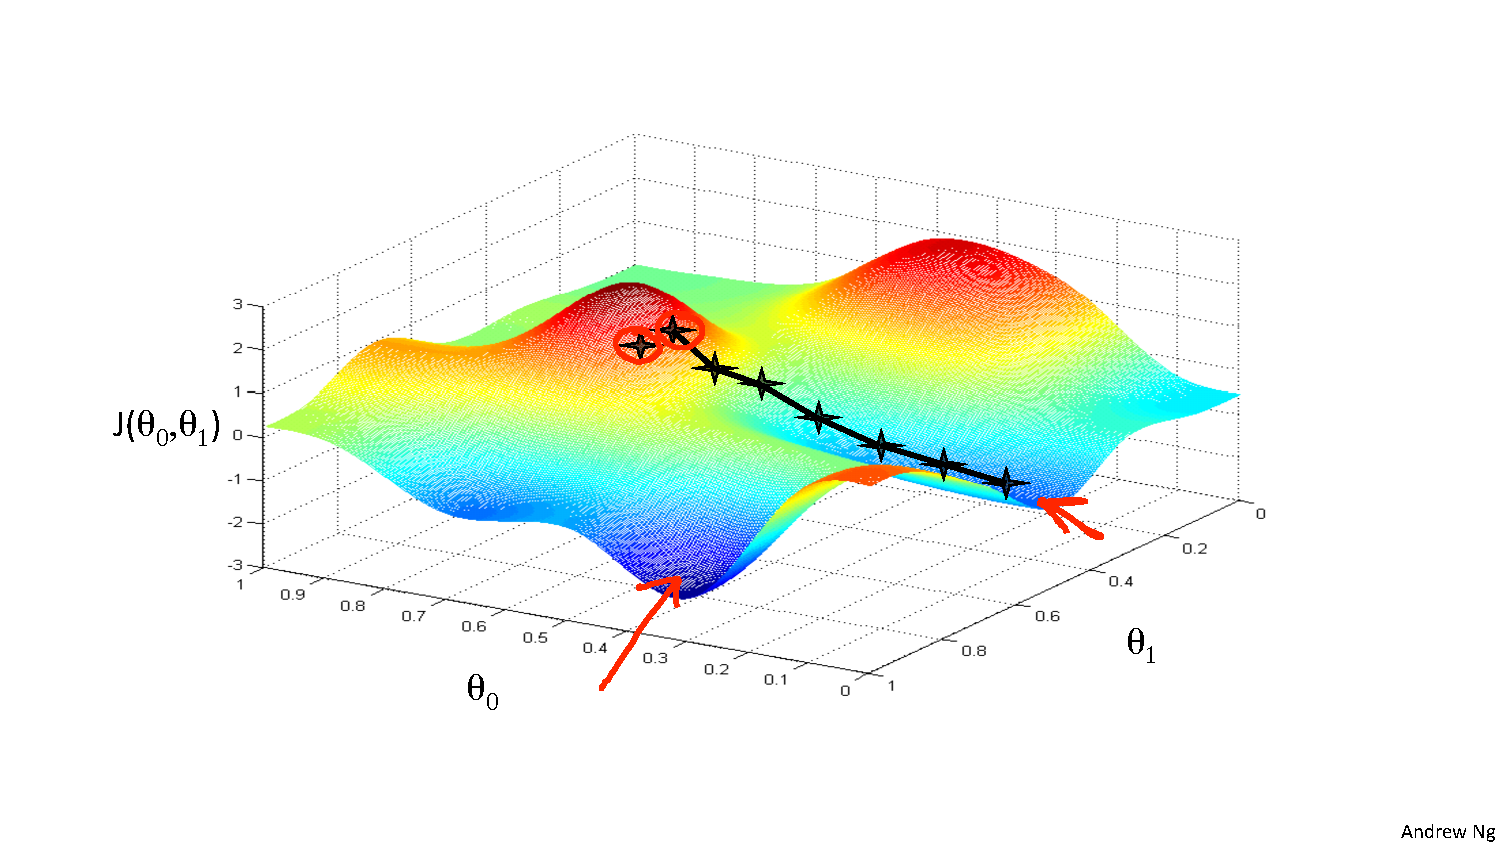
\includegraphics[width=\linewidth,trim=40pt 48pt 70pt 55pt,clip]{assets/andrew-ng-cost-landscape.pdf}
  \par\smallskip
  {\small\textit{A function with several valleys. Source:
  \href{https://d396qusza40orc.cloudfront.net/ml/docs/slides/Lecture2.pdf}
  {Andrew Ng, Machine Learning, Lecture 2, slide 25}.}}
\end{center}

Here the function has two inputs: the adjustable parameters $\theta_0$
and $\theta_1$ on the horizontal axes. The height $J(\theta_0,\theta_1)$
is the value we want to minimise; $J$ plays the same role as $g$ in
our notation. The black path shows successive downhill steps into
the valley on the right. The valley in front is deeper: being lower
than nearby points does not necessarily mean having the lowest value
overall.

\begin{frameddefn}{Local minimum and local maximum}\label{def:local-optimum}
An input $w_*$ is a \emph{local minimum point} if
\[
  g(w_*)\leq g(w)\qquad\text{for all }w\text{ sufficiently near }w_*.
\]
It is a \emph{local maximum point} if the inequality is reversed.
Here ``sufficiently near'' means that the comparison holds throughout
some small interval around $w_*$.
\end{frameddefn}

\Needspace{30\baselineskip}
\begin{framedexample}{Valleys of different depths}
Consider the sum of an oscillating function and a quadratic term:
\[
  g(w)=\sin(3w)+0.1w^2.
\]
The sine term produces peaks and valleys. The quadratic term grows
as $|w|$ increases, so these valleys have different depths. The graph
shows two of them with colored dots.

\begin{center}
\begin{tikzpicture}[font=\small,x=1.4cm,y=1.2cm]
  \draw[-{Stealth},black!50] (-3.3,0)--(3.5,0) node[right] {$w$};
  \draw[-{Stealth},black!50] (0,-1.3)--(0,2) node[above] {$g(w)$};
  \draw[NotesBlue,thick,domain=-3:3,samples=181]
    plot (\x,{sin(deg(3*\x))+0.1*\x*\x});
  \foreach \xx in {-3,-2,-1,1,2,3} {
    \draw[black!50] (\xx,0.06)--(\xx,-0.06) node[below] {$\xx$};
  }
  \node[below left] at (0,0) {$0$};
  \fill[green!60!black] (-0.512214,-0.973180) circle (2.5pt);
  \node[below left] at (-0.512214,-0.973180) {$w\approx-0.5$};
  \fill[orange!90!black] (1.536590,-0.758628) circle (2.5pt);
  \node[below right] at (1.536590,-0.758628) {$w\approx1.5$};
\end{tikzpicture}
\end{center}

The green point near $w=-0.5$ is the deepest valley: its value is
about $-0.973$. It is a global minimum point. The orange point near
$w=1.5$ is also lower than its immediate neighbors, but its value is
about $-0.759$. It is a local minimum point with a larger objective
value.

The peaks near $w\approx0.536$ and $w\approx2.678$ are local maximum
points: their values are larger than those at nearby inputs.
\end{framedexample}

Imagine searching for a minimum by making small changes that lower
$g$. In this example, the search can stop in the orange valley.
Reaching the deeper green valley requires first climbing out of the
orange one. The orange point is a local minimum, but the green point
has a lower value of $g$.

\Needspace{8\baselineskip}
\section{Why these are called zero-order conditions}

The global and local definitions compare values of $g$ directly.
They are called \emph{zero-order conditions} because they use the
function itself. First-order conditions use first derivatives, which
describe the slope of the graph. Second-order conditions use second
derivatives, which describe how that slope changes. The definitions
tell us what it means to be a minimum or maximum; derivatives will
help us find candidate optimum points without comparing every
possible input individually.

\clearpage
\section{Using the derivative to find candidate optima}

We now want to find possible minimum points by solving an equation.
With one adjustable number $w$, we use the derivative $g'(w)$, also
written $\frac{\mathrm{d}g}{\mathrm{d}w}$. It tells us how $g$ changes
when we change $w$ slightly. On the graph, it is the slope of the
\emph{tangent line}: the straight line that follows the direction
of the curve at the point we are examining.

If $g'(w)>0$, moving slightly to the right increases $g$.
If $g'(w)<0$, the same movement decreases $g$.
If $g'(w)=0$, the tangent is horizontal. Let us see what happens
at the bottom of a parabola.

\Needspace{25\baselineskip}
\begin{framedexample}{A horizontal tangent at the minimum}
Suppose we want to minimise $g(w)=w^2+1$. The blue curve shows
the objective, and the green line is its tangent at $w=0$.

\begin{center}
\begin{tikzpicture}[font=\small,x=1.25cm,y=0.65cm]
  \draw[-{Stealth},black!50] (-2.4,0)--(2.6,0) node[right] {$w$};
  \draw[-{Stealth},black!50] (0,-0.3)--(0,5.6) node[above] {$g(w)$};
  \draw[NotesBlue,thick,domain=-2:2,samples=81]
    plot (\x,{\x*\x+1});
  \draw[green!60!black,thick] (-1.7,1)--(1.7,1);
  \node[green!50!black,right] at (1.7,1) {slope $0$};
  \fill[green!60!black] (0,1) circle (2.5pt);
  \node[below left] at (0,0) {$0$};
  \node[above left] at (0,1) {$1$};
\end{tikzpicture}
\end{center}

Differentiate $w^2$ to obtain $2w$; the constant $1$ contributes
zero. To find where the slope is zero, solve
\[
  g'(w)=2w=0\qquad\Longrightarrow\qquad w_*=0.
\]
This point is a global minimum because $w^2+1\geq1$ for every $w$,
and $g(0)=1$.
\end{framedexample}

Assume that the derivative exists and that we can move a little
to either side of the input. At a local minimum, neither direction
can lower $g$. A nonzero slope would let us lower it by moving in
one of those directions. The slope must therefore be zero.

\begin{frameddefn}{Stationary point and first-order condition}\label{def:first-order-scalar}
An input $w_*$ is a \emph{stationary point} if
\[
  g'(w_*)=0.
\]
For a differentiable function, every local minimum or local maximum
inside the input domain satisfies this equation. It is called the
\emph{first-order condition}. Here ``inside'' means that small moves
to both sides are allowed.
\end{frameddefn}

\clearpage
\section{Why a zero derivative is not enough}

Solving $g'(w)=0$ gives us points to check. A horizontal tangent
can occur at a minimum, at a maximum, or at a point that is neither.
The next three curves show these possibilities.

\Needspace{34\baselineskip}
\begin{framedexample}{Three stationary points with different meanings}
Consider $g(w)=w^2$, $g(w)=-w^2$, and $g(w)=w^3$.
Each graph has a horizontal tangent at $w=0$.

\begin{center}
\begin{tikzpicture}[font=\small,x=1cm,y=0.65cm]
  \begin{scope}
    \node at (0,2.8) {$g(w)=w^2$};
    \draw[-{Stealth},black!50] (-1.5,0)--(1.65,0) node[right] {$w$};
    \draw[-{Stealth},black!50] (0,-2.2)--(0,2.2);
    \draw[NotesBlue,thick,domain=-1.25:1.25,samples=81]
      plot (\x,{\x*\x});
    \draw[green!60!black,thick] (-0.7,0)--(0.7,0);
    \fill[green!60!black] (0,0) circle (2.5pt);
    \node[below left] at (0,0) {$0$};
    \node at (0,-2.8) {minimum};
  \end{scope}
  \begin{scope}[xshift=4.5cm]
    \node at (0,2.8) {$g(w)=-w^2$};
    \draw[-{Stealth},black!50] (-1.5,0)--(1.65,0) node[right] {$w$};
    \draw[-{Stealth},black!50] (0,-2.2)--(0,2.2);
    \draw[NotesBlue,thick,domain=-1.25:1.25,samples=81]
      plot (\x,{-\x*\x});
    \draw[green!60!black,thick] (-0.7,0)--(0.7,0);
    \fill[orange!90!black] (0,0) circle (2.5pt);
    \node[below left] at (0,0) {$0$};
    \node at (0,-2.8) {maximum};
  \end{scope}
  \begin{scope}[xshift=9cm]
    \node at (0,2.8) {$g(w)=w^3$};
    \draw[-{Stealth},black!50] (-1.5,0)--(1.65,0) node[right] {$w$};
    \draw[-{Stealth},black!50] (0,-2.2)--(0,2.2);
    \draw[NotesBlue,thick,domain=-1.25:1.25,samples=81]
      plot (\x,{\x*\x*\x});
    \draw[green!60!black,thick] (-0.7,0)--(0.7,0);
    \fill[black] (0,0) circle (2.5pt);
    \node[below left] at (0,0) {$0$};
    \node at (0,-2.8) {neither};
  \end{scope}
\end{tikzpicture}
\end{center}

For $g(w)=w^2$, solving $g'(w)=2w=0$ gives $w=0$.
Every value of $w^2$ is nonnegative, so this is a minimum.

For $g(w)=-w^2$, solving $g'(w)=-2w=0$ also gives $w=0$.
Every value of $-w^2$ is nonpositive, so this is a maximum.

For $g(w)=w^3$, the first-order equation is
\[
  g'(w)=3w^2=0\qquad\Longrightarrow\qquad w=0.
\]
Choose any small positive number $\varepsilon$. On opposite sides
of $0$, the function takes values
\[
  g(-\varepsilon)=-\varepsilon^3<g(0)=0
  <\varepsilon^3=g(\varepsilon).
\]
We can make these inputs as close to $0$ as we want. There are
therefore both smaller and larger values near $0$, so it is neither
a minimum nor a maximum. It is a \emph{stationary point of inflection}:
the tangent is horizontal and the curve changes how it bends,
but it keeps rising through the point.
\end{framedexample}

The first-order condition is \emph{necessary} at a differentiable
interior minimum, but it is not \emph{sufficient}: every such minimum
has zero derivative, while some points with zero derivative are not
minima. We must still examine the function around each candidate.

\clearpage
\section{Several weights: a system of first-order equations}

We now make the same search with several adjustable weights.
Write them as the vector $w=(w_1,\ldots,w_N)^\top$, where $N$ is
the number of weights. The objective $g(w)$ still returns a single
score, but that score now depends on all $N$ entries.

To check the effect of one weight, vary $w_j$ while keeping the
others fixed. The resulting rate of change is the \emph{partial
derivative} $\frac{\partial g}{\partial w_j}$. The index $j$ identifies
the weight being varied, from $1$ to $N$.

\begin{frameddefn}{Gradient}\label{def:optimization-gradient}
For a differentiable function $g$ of $N$ weights, the \emph{gradient}
collects its $N$ partial derivatives in one column vector:
\[
  \nabla g(w)=
  \begin{pmatrix}
    \dfrac{\partial g}{\partial w_1}(w)\\[4pt]
    \dfrac{\partial g}{\partial w_2}(w)\\
    \vdots\\
    \dfrac{\partial g}{\partial w_N}(w)
  \end{pmatrix}.
\]
The $j$th entry measures how $g$ changes when we vary $w_j$ while
keeping the other weights fixed.
\end{frameddefn}

At a differentiable local minimum inside the input domain, every
entry must be zero. Otherwise, changing one weight in the appropriate
direction would lower the score.

\begin{frameddefn}{First-order system}\label{def:first-order-system}
A stationary point $w_*$ satisfies the $N$ equations
\[
  \begin{cases}
    \dfrac{\partial g}{\partial w_1}(w_*)=0,\\[5pt]
    \dfrac{\partial g}{\partial w_2}(w_*)=0,\\
    \hfill\vdots\\
    \dfrac{\partial g}{\partial w_N}(w_*)=0.
  \end{cases}
  \qquad\Longleftrightarrow\qquad
  \nabla g(w_*)=\mathbf{0}_{N\times1}.
\]
The right-hand side is a column vector of $N$ zeros. The equations
set every partial derivative to zero, not the value of $g$.
\end{frameddefn}

When we can solve these equations directly, we obtain an
\emph{analytic solution}, also called a \emph{closed-form solution}.
The next example shows the calculation with two weights.

\Needspace{34\baselineskip}
\begin{framedexample}{Two weights, two equations}
Suppose we want to minimise
\[
  g(w_1,w_2)=(w_1-1)^2+(w_2+2)^2+1.
\]
The surface is a bowl. The green plane is its horizontal tangent
at the green point $(w_1,w_2)=(1,-2)$.

\begin{center}
\begin{tikzpicture}
\begin{axis}[
  width=10cm,height=6cm,view={135}{25},
  xlabel={$w_1$},ylabel={$w_2$},zlabel={$g(w_1,w_2)$},
  label style={font=\small},tick label style={font=\small},
  xmin=-0.5,xmax=2.5,ymin=-3.5,ymax=-0.5,zmin=0,zmax=5.5,
  xtick={0,1,2},ytick={-3,-2,-1},ztick={1,3,5},
  domain=-0.5:2.5,y domain=-3.5:-0.5,
  axis lines=box,grid=major,grid style={black!12}]
  \addplot3[surf,shader=flat,opacity=0.5,samples=2,
    domain=-0.2:2.2,y domain=-3.2:-0.8,
    colormap={FlatTangent}{color=(NotesDefinition) color=(NotesDefinition)}]
    {1};
  \addplot3[mesh,thin,samples=15,
    colormap={NotesBowl}{color=(NotesBlue) color=(NotesBlue)}]
    {(x-1)^2+(y+2)^2+1};
  \addplot3[only marks,mark=*,mark size=2.5pt,green!60!black]
    coordinates {(1,-2,1)};
\end{axis}
\end{tikzpicture}
\end{center}

Differentiate with respect to $w_1$, keeping $w_2$ fixed. The term
$(w_2+2)^2$ is then constant and contributes zero. Reversing the roles
of the weights gives the other partial derivative:
\[
  \frac{\partial g}{\partial w_1}=2(w_1-1),\qquad
  \frac{\partial g}{\partial w_2}=2(w_2+2).
\]
Set both equal to zero and solve the two equations:
\[
  \begin{cases}
    2(w_1-1)=0\quad\Longrightarrow\quad w_1=1,\\
    2(w_2+2)=0\quad\Longrightarrow\quad w_2=-2.
  \end{cases}
\]
Thus $w_*=(1,-2)^\top$. Both squares vanish there, so $g(w_*)=1$.
Every other value is at least $1$: this candidate is a global minimum.
\end{framedexample}

\clearpage
With several weights, a zero gradient can also identify a point
that is neither a minimum nor a maximum. One direction may lead
to larger values while another leads to smaller ones.

\begin{frameddefn}{Saddle point}\label{def:saddle-point}
A \emph{saddle point} of a differentiable function is a stationary
point with both smaller and larger function values arbitrarily
nearby. It is therefore neither a local minimum nor a local maximum.
\end{frameddefn}

\Needspace{28\baselineskip}
\begin{framedexample}{Zero gradient at a saddle point}
Consider the two-weight objective $g(w_1,w_2)=w_1^2-w_2^2$.
Its first-order equations are
\[
  \frac{\partial g}{\partial w_1}=2w_1=0,\qquad
  \frac{\partial g}{\partial w_2}=-2w_2=0.
\]
They give the stationary point $w_*=(0,0)^\top$, with $g(w_*)=0$.
To examine this point, let $t$ be a small change in one weight.
The graph shows the function along the two coordinate directions:
$g(t,0)=t^2$ when we change only $w_1$, and $g(0,t)=-t^2$ when
we change only $w_2$.

\begin{center}
\begin{tikzpicture}[font=\small,x=1.5cm,y=0.8cm]
  \draw[-{Stealth},black!50] (-1.8,0)--(2,0) node[right] {$t$};
  \draw[-{Stealth},black!50] (0,-2.3)--(0,2.5) node[above] {objective value};
  \draw[NotesBlue,thick,domain=-1.4:1.4,samples=81]
    plot (\x,{\x*\x});
  \draw[orange!90!black,thick,domain=-1.4:1.4,samples=81]
    plot (\x,{-\x*\x});
  \node[NotesBlue,right] at (1.4,1.96) {$g(t,0)=t^2$};
  \node[orange!90!black,right] at (1.4,-1.96) {$g(0,t)=-t^2$};
  \fill[black] (0,0) circle (2.5pt);
  \node[below left] at (0,0) {$0$};
\end{tikzpicture}
\end{center}

For any nonzero $t$, changing only $w_1$ raises the value above $0$,
while changing only $w_2$ lowers it below $0$. These changes can be
as small as we want. The point $(0,0)^\top$ is a saddle point,
even though both partial derivatives are zero.
\end{framedexample}

\clearpage
\section{Approximating a function near one point}

Solving $g'(w)=0$ can become difficult when $g$ is complicated.
Another useful way to study the objective is to replace a small part
of its graph with a simpler shape: its tangent line. This approximation
helps us predict how a small change in a weight will affect the score.

Choose a starting input $w_0$. We know the value $g(w_0)$ and the
slope $g'(w_0)$ there. Moving from $w_0$ to a nearby input $w$ changes
the input by $w-w_0$. Multiplying this change by the slope gives the
predicted change in the function.

\begin{frameddefn}{First-order Taylor approximation}\label{def:first-order-taylor}
The \emph{first-order Taylor approximation} of $g$ at $w_0$ is
\[
  h(w)=g(w_0)+g'(w_0)(w-w_0).
\]
The function $h$ is the tangent line. It has the same value and the
same slope as $g$ at $w_0$. For inputs close to $w_0$, we use
$g(w)\approx h(w)$.
\end{frameddefn}

\Needspace{26\baselineskip}
\begin{framedexample}{Using a tangent line to predict a nearby value}
Take $g(w)=w^2+1$ and choose $w_0=1$. The green line touches the
blue curve at $(1,2)$ and follows its slope there.

\begin{center}
\begin{tikzpicture}[font=\small,x=1.8cm,y=0.6cm]
  \draw[-{Stealth},black!50] (-0.3,0)--(2.7,0) node[right] {$w$};
  \draw[-{Stealth},black!50] (0,-0.3)--(0,6.7) node[above] {value};
  \draw[NotesBlue,thick,domain=0:2.3,samples=81]
    plot (\x,{\x*\x+1});
  \draw[green!60!black,thick] (0,0)--(2.3,4.6);
  \draw[black!35,dashed] (1,0)--(1,2)--(0,2);
  \fill[green!60!black] (1,2) circle (2.5pt);
  \node[below] at (1,0) {$w_0=1$};
  \node[left] at (0,2) {$2$};
  \node[NotesBlue,right] at (2.3,6.29) {$g(w)$};
  \node[green!50!black,right] at (2.3,4.6) {$h(w)$};
\end{tikzpicture}
\end{center}

At the chosen input, $g(1)=2$ and $g'(1)=2$. Substituting these
numbers into the approximation gives
\[
  h(w)=2+2(w-1)=2w.
\]
For the nearby input $w=1.1$, the line predicts $h(1.1)=2.2$.
The actual value is $g(1.1)=1.1^2+1=2.21$, so the prediction is close.

Farther away, at $w=2$, the line predicts $4$, while the function
gives $5$. The tangent describes the function near the chosen point;
it does not replace the whole curve.
\end{framedexample}

\clearpage
\subsection{From a tangent line to a tangent plane}

With $N$ weights, the starting input $w_0$ is a vector.
The displacement $w-w_0$ contains the change in each weight.
Each partial derivative predicts the effect of its corresponding
change, and we add these contributions:
\[
  \nabla g(w_0)^\top(w-w_0)
  =\sum_{j=1}^{N}\frac{\partial g}{\partial w_j}(w_0)
    (w_j-w_{0,j}).
\]
Here $w_{0,j}$ is the $j$th entry of the starting vector $w_0$.
The product on the left is a dot product: it multiplies matching
entries of the two vectors and sums the results.

\begin{frameddefn}{Tangent hyperplane}\label{def:tangent-hyperplane}
For a differentiable function of several weights, the first-order
Taylor approximation at $w_0$ is
\[
  h(w)=g(w_0)+\nabla g(w_0)^\top(w-w_0).
\]
Its graph is the \emph{tangent hyperplane}. It passes through the
point $(w_0,g(w_0))$ and has the same partial derivatives as $g$
there. For nearby inputs, $g(w)\approx h(w)$.
\end{frameddefn}

For one input, the graph is a line with two coordinates: the weight
and the function value. For two inputs, it is a plane with three
coordinates: two weights and the function value. In general, this
flat graph has dimension $N$ in a space with $N+1$ coordinates.

We can collect the constants and write the same model as
\[
  h(w)=a+b^\top w,\qquad
  a=g(w_0)-\nabla g(w_0)^\top w_0,\quad b=\nabla g(w_0).
\]
The vector $b$ contains the slopes, while the scalar $a$ sets the
height of the graph when $w=0$. This is an \emph{affine hyperplane}:
the constant term allows it to be shifted away from the origin.

\Needspace{32\baselineskip}
\begin{framedexample}{A tangent plane for two weights}
Use the objective $g(w_1,w_2)=(w_1-1)^2+(w_2+2)^2+1$ and
choose the starting weights $w_0=(2,-1)^\top$. The green plane
touches the blue surface at this point.

\begin{center}
\begin{tikzpicture}
\begin{axis}[
  width=10cm,height=6cm,view={45}{25},
  xlabel={$w_1$},ylabel={$w_2$},zlabel={value},
  label style={font=\small},tick label style={font=\small},
  xmin=0.5,xmax=3.5,ymin=-2.5,ymax=0.5,zmin=-1,zmax=14,
  xtick={1,2,3},ytick={-2,-1,0},ztick={0,3,6,9,12},
  domain=0.5:3.5,y domain=-2.5:0.5,
  axis lines=box,grid=major,grid style={black!12}]
  \addplot3[surf,shader=flat,opacity=0.65,draw=green!60!black,samples=2,
    domain=1:3,y domain=-2:0,
    colormap={SlopingTangent}{color=(NotesDefinition) color=(NotesDefinition)}]
    {1+2*x+2*y};
  \addplot3[mesh,thin,samples=15,
    colormap={SecondBowl}{color=(NotesBlue) color=(NotesBlue)}]
    {(x-1)^2+(y+2)^2+1};
  \addplot3[only marks,mark=*,mark size=2.5pt,green!60!black]
    coordinates {(2,-1,3)};
\end{axis}
\end{tikzpicture}
\end{center}

First compute the function value and the partial derivatives at
the starting weights:
\[
  g(2,-1)=1^2+1^2+1=3,\qquad
  \nabla g(2,-1)=
  \begin{pmatrix}2(2-1)\\2(-1+2)\end{pmatrix}
  =\begin{pmatrix}2\\2\end{pmatrix}.
\]
The tangent model is therefore
\[
  h(w_1,w_2)=3+2(w_1-2)+2(w_2+1)=1+2w_1+2w_2.
\]
In the form $h(w)=a+b^\top w$, we have $a=1$ and $b=(2,2)^\top$.
Checking the starting point gives $h(2,-1)=3$, exactly as required.

Changing both weights by $0.1$ gives $(2.1,-0.9)^\top$.
The plane predicts $3.4$, while the actual function value is
$1.1^2+1.1^2+1=3.42$.
\end{framedexample}

\clearpage
\section{Choosing the direction of fastest change}

The tangent model helps us choose how to change several weights
together. With one weight, we can move left or right; the sign of
the slope determines which way increases the function. With two
or more weights, there are infinitely many directions to consider.

Let $d=(d_1,\ldots,d_N)^\top$ describe a direction. To compare
directions fairly, give them the same Euclidean length:
\[
  \|d\|=\sqrt{d_1^2+\cdots+d_N^2}=1.
\]
Such a vector is called a \emph{unit direction}. If $\alpha>0$ is
the distance we choose to move, the new weights are $w_0+\alpha d$.
All the directions being compared then produce steps of length
$\alpha$.

For the affine model $h(w)=a+b^\top w$, this move gives
\[
  h(w_0+\alpha d)=a+b^\top w_0+\alpha b^\top d.
\]
The first two terms are fixed. The predicted change is
$\alpha b^\top d$, so the direction with the largest dot product
$b^\top d$ gives the largest increase; the smallest gives the largest
decrease.

Assume $b\ne0$ and let $\theta$ be the angle between $b$ and $d$.
The dot product satisfies
\[
  b^\top d=\|b\|\,\|d\|\cos\theta=\|b\|\cos\theta.
\]
The length $\|b\|$ is fixed. The largest value occurs when
$\cos\theta=1$, so $d$ points along $b$. The smallest occurs when
$\cos\theta=-1$, so $d$ points opposite to $b$.

\begin{frameddefn}{Steepest ascent and steepest descent}\label{def:steepest-directions}
At an input $w_0$ where $\nabla g(w_0)\ne0$, the Euclidean unit
directions of fastest local increase and decrease are
\[
  d_{\mathrm{ascent}}=
  \frac{\nabla g(w_0)}{\|\nabla g(w_0)\|},\qquad
  d_{\mathrm{descent}}=
  -\frac{\nabla g(w_0)}{\|\nabla g(w_0)\|}.
\]
The largest rate of increase per unit distance is $\|\nabla g(w_0)\|$.
The gradient itself points in the ascent direction, and its negative
points in the descent direction. Dividing by the length makes these
vectors unit directions.
\end{frameddefn}

The tangent model has the same slopes as the original function at
$w_0$, so these are also the fastest \emph{local} directions for $g$.
A sufficiently small step opposite to a nonzero gradient lowers $g$;
a large step can increase it. Choosing a direction and choosing how
far to move are therefore separate parts of the search.

At a stationary point, the gradient is zero and the tangent model
is horizontal. It gives no preferred direction: we must examine more
than this first-order approximation to understand the function there.

\Needspace{32\baselineskip}
\begin{framedexample}{Equal step lengths, different changes}
For $g(w_1,w_2)=(w_1-1)^2+(w_2+2)^2+1$ at $w_0=(2,-1)^\top$,
the tangent model is $h(w)=1+2w_1+2w_2$ and $b=(2,2)^\top$.
Compare the following unit directions. The dot product gives the
change in $h$ per unit distance.

\begin{center}
\begin{tabular}{ccc}
\toprule
Unit direction $d$ & $b^\top d$ & Effect on $h$\\
\midrule
$(1,0)^\top$ & $2$ & increase\\[3pt]
$(0,1)^\top$ & $2$ & increase\\[3pt]
$(1,-1)^\top/\sqrt{2}$ & $0$ & no change\\[3pt]
$(1,1)^\top/\sqrt{2}$ & $2\sqrt{2}$ & fastest increase\\[3pt]
$(-1,-1)^\top/\sqrt{2}$ & $-2\sqrt{2}$ & fastest decrease\\
\bottomrule
\end{tabular}
\end{center}

The gradient length is $\sqrt{2^2+2^2}=2\sqrt{2}$. Dividing the
negative gradient by this length gives
\[
  d_{\mathrm{descent}}=
  \frac{1}{\sqrt{2}}\begin{pmatrix}-1\\-1\end{pmatrix}.
\]
A step of length $\alpha$ in this direction gives the new weights
\[
  w_0+\alpha d_{\mathrm{descent}}
  =\begin{pmatrix}2-\alpha/\sqrt{2}\\-1-\alpha/\sqrt{2}\end{pmatrix}.
\]
The tangent model predicts the value $3-2\sqrt{2}\alpha$.
Substituting the new weights into the actual objective gives
\[
  g(w_0+\alpha d_{\mathrm{descent}})
  =2\left(1-\frac{\alpha}{\sqrt{2}}\right)^2+1
  =3-2\sqrt{2}\alpha+\alpha^2.
\]
For $\alpha=0.1$, the predicted value is about $2.717$, and the
actual value is about $2.727$. Both are below the starting value $3$.
The extra $\alpha^2$ term shows the part that the tangent model
does not capture.
\end{framedexample}

\clearpage
\section{Level curves and the gradient}

We can also view a two-weight objective from above. Instead of
drawing its height, we connect inputs with the same function value,
as a map connects places at the same altitude.

\begin{frameddefn}{Level set and level curve}\label{def:level-set}
For a fixed score $c$, the \emph{level set} of $g$ is
\[
  \{w:g(w)=c\}.
\]
With two inputs, these sets are usually drawn as \emph{level curves}.
Every point on one curve has the same score $c$. Different curves
correspond to different scores.
\end{frameddefn}

\Needspace{32\baselineskip}
\begin{framedexample}{Reading the gradient on a contour map}
For $g(w_1,w_2)=(w_1-1)^2+(w_2+2)^2+1$, the level curves are
circles centred at the minimum $(1,-2)^\top$, where $g=1$.
The black point $w_0=(2,-1)^\top$ has score $3$.

\begin{center}
\begin{tikzpicture}[font=\small,x=1cm,y=1cm]
  \draw[-{Stealth},black!35] (-1.4,0)--(3.8,0) node[right] {$w_1$};
  \draw[-{Stealth},black!35] (0,-4.4)--(0,0.7) node[above] {$w_2$};
  \foreach \rr in {1,1.414214,2}
    {\draw[NotesBlue!70,thick] (1,-2) circle (\rr);}
  \node[fill=NotesPaper,inner sep=1pt,right] at (1.6,-2.8) {$g=2$};
  \node[fill=NotesPaper,inner sep=1pt,right] at (1.2,-3.4) {$g=3$};
  \node[fill=NotesPaper,inner sep=1pt,right] at (2.6,-3.2) {$g=5$};
  \fill[green!60!black] (1,-2) circle (2.5pt);
  \node[below left] at (1,-2) {$g=1$};
  \draw[black!55,dashed] (1.4,-0.4)--(2.6,-1.6);
  \draw[black!55,thin] (1.2,0.05)--(1.4,-0.4);
  \node[above left] at (1.4,0.05) {tangent};
  \draw[-{Stealth},orange!90!black,thick] (2,-1)--(2.8,-0.2);
  \node[orange!90!black,right] at (2.8,-0.2) {ascent};
  \draw[-{Stealth},green!60!black,thick] (2,-1)--(1.45,-1.55);
  \node[green!50!black,below right] at (1.45,-1.55) {descent};
  \draw[black!70] (2.12,-0.88)--(2.24,-1)--(2.12,-1.12);
  \fill[black] (2,-1) circle (2.5pt);
  \node[above left] at (2,-1) {$w_0$};
\end{tikzpicture}
\end{center}

The gradient $(2,2)^\top$ points outward, towards larger scores;
its negative points inward, towards smaller scores.
The dashed tangent direction $t=(1,-1)^\top$ is perpendicular to it:
\[
  \nabla g(w_0)^\top t=2\cdot1+2\cdot(-1)=0.
\]
Moving along the level curve keeps the score constant, so the
first-order change in its tangent direction is zero.
\end{framedexample}

Where the gradient is nonzero, it is perpendicular to the level
curve. In higher dimensions, it is perpendicular to the surface
of constant function value.

\smallskip
{\small\textit{Sources: Spinelli, Lecture 03 (Optimization), slides 2--29;
Watt, Borhani, and Katsaggelos, Machine Learning Refined (2016),
Sections 1.4, 2.1.1--2.1.2, and 2.2.1.}}

\end{document}
